%\documentclass[a4paper]{article}
\documentclass[usenatbib]{mn2e}
%% Language and font encodings
\usepackage[english]{babel}
\usepackage[utf8x]{inputenc}
\usepackage[T1]{fontenc}
\usepackage{lineno}
\linenumbers
\modulolinenumbers[2]

\usepackage{natbib}
%% Sets page size and margins
\usepackage[a4paper,top=3cm,bottom=2cm,left=3cm,right=3cm,marginparwidth=1.75cm]{geometry}

%% Useful packages
\usepackage{amsmath}
\usepackage{amsfonts}
\usepackage{graphicx}
\usepackage{subcaption}
\usepackage[colorinlistoftodos]{todonotes}
\usepackage[colorlinks=true, allcolors=blue]{hyperref}
\usepackage{multirow}

\newcommand       \apj  {ApJ}
\newcommand       \apjl  {ApJL}
\newcommand       \apjs  {ApJS}
\newcommand       \aj  {AJ}
\newcommand       \aap {A\&A}
\newcommand       \mnras {MNRAS}
\newcommand       \nat {Nature}
\newcommand       \araa {ARA\&A}
\newcommand       \physrep {Phys.~Reports}
\newcommand       \prd {Phys. Rev. D}

\newcommand{\trainz}{\textsc{trainZ}}

\newcommand{\textul}{\underline}
\newcommand*\mathinhead[2]{\texorpdfstring{$\boldsymbol{#1}$}{#2}}

\newcommand{\red}[1]{\textcolor{red}{#1}}
% Claim a color for your comments
\newcommand{\aim}[1]{\textcolor{green}{#1}}%Alex Malz comments in green
\newcommand{\blue}[1]{\textcolor{blue}{#1}}%unknown person comments in blue
\definecolor{scc}{rgb}{0.0, 0.26, 0.15}
\newcommand{\scc}[1]{\textcolor{scc}{#1}}%Stefano Cavuoti Comments in dark green
\definecolor{newpink}{rgb}{0.858, 0.188, 0.478}
\newcommand{\erfan}[1]{\textcolor{newpink}{#1}} % Erfan Nourbakhsh comments in pink
\newcommand{\jan}[1]{\textcolor{orange}{#1}}%Alex Malz comments in green

\def\X{{\mathbf{X}}}
\def\x{{\mathbf{x}}}
\def\E{{\mathbb E}}

\title{An assessment of photometric redshift PDF performance in the context of LSST}
% Alternate title proposal: Assessing the characterization of photometric redshift uncertainties in the regime of LSST

\author{LSST-DESC Photometric Redshift Working Group}

\begin{document}
\maketitle

\begin{abstract}
Photometric redshift (photo-$z$) probability distribution functions (PDFs) are a key data product of nearly all upcoming galaxy imaging surveys.
However, the photo-$z$ PDFs resulting from different techniques are not in general consistent with one another, and an optimal method for obtaining an accurate PDF remains unclear.  
We present the results of an initial study of the Large Synoptic Survey Telescope Dark Energy Science Collaboration (LSST-DESC), the first in a planned series of papers testing multiple photo-$z$ codes on simulations of upcoming LSST galaxy photometry catalogues.  This initial test evaluates photo-$z$ algorithms in the presence of representative training data and in the absence of several common sources of systematic errors that affect the procedures by which photo-$z$ PDFs are derived.  
The photo-$z$ PDFs are evaluated using multiple metrics including the Kolmogorov-Smirnoff statistic, Cramer-von Mises statistic, Anderson-Darling statistic, Kullback-Leibler divergence, $N(z)$ moments, quantile-quantile plots and probability integral transform.  We observe several trends, including an overall over/under-prediction in the broadness of the PDFs for several of the codes.  A careful accounting of all systematics discovered will be necessary for the codes employed in upcoming analyses in order to achieve unbiased cosmological measurements.
\end{abstract}
\begin{keywords}
galaxies: distances and redshifts -- galaxies: statistics -- methods: statistical
\end{keywords}
%\noindent comments color-code:\\
%\red{SJS},
%\aim{AIM},
%\scc{SC},
%\textcolor{brown}{MB},\jan{JAN}
%\blue{unknown}\\
%\red{note: not all red text is mine, at some point various people were using red --SJS.}


% Questions left unanswered:
% 1. Which journal will this paper be published? 
% Answer: AJ / ApJ / MNRAS (no charges, but not sure if it will accept a paper based on a DC1 effort and the associated simulations)
% 2. What is the meaning of $p(z)$ in different codes? (Ofer)
% Answer: ?
%

\section{Introduction}
\label{sec:intro}

%(Sam Schmidt, Ofer Lahav, Jeff Newman, Alex Malz, John Soo, Tony Tyson)

%\jan{Is the intention to keep these parenthetical author sets?  I find it a bit offputting in the text.  It might be better to put this for sections in the acknowledgements section, and for individual codes/statistics specify who ran/developed it with a sentence.}\red{I was just about to comment these out before finalizing the internal review draft of the paper. They are in place to remind me to contact a few people who still have not filled out their authors.csv info.}

Large-scale photometric galaxy surveys are entering a new era with currently or soon-to-be running Stage III and Stage IV dark energy experiments like the Dark Energy Survey \citep[DES,][]{Abbott:05}, the Kilo-Degree Survey \citep[KiDS,][]{de_Jong:13}, Large Synoptic Survey Telescope \citep[LSST,][]{Abell:09}, Euclid \citep{Laureijs:11}, and Wide-Field Infrared Survey Telescope \citep[WFIRST,][]{Green:12}. 
The move to imaging based surveys, rather than spectroscopic based, for cosmological measurements makes proper understanding of photometric redshifts (``photo-$z$'s'') of paramount importance, as cosmological distance measures for statistical samples are directly dependent on photo-$z$ measurements.  

The unprecedented sample size of LSST galaxies, expected to number several billion for the main cosmological sample, necessitates stringent constraints on photo-$z$ accuracy if systematic errors are not to dominate the statistical errors. 
The LSST Science Requirements Document (SRD)\footnote{available at \url{https://docushare.lsstcorp.org/docushare/dsweb/Get/LPM-17}} lists the photometric redshift goals for a magnitude limited sample with $i<25$ as: root-mean-square error with a goal of $\sigma_z<0.02(1+z)$; $3\sigma$ ``catastrophic outlier'' rate below $10\%$; bias below $0.003$\footnote{ 
Note that at the time the SRD was written, these goals were stated in terms of a photo-$z$ point estimate for each galaxy, as was standard in many previous studies, while in this paper we emphasize the importance of using a full photo-$z$ PDF.}.  

The tremendous size of LSST's galaxy catalog will be enabled by its exceptional depth, pushing to fainter magnitudes and deeper imaging and including galaxies of lower luminosity and higher redshift than ever before. 
In addition to the contribution of low signal-to-noise photometry to the systematic error of photo-$z$s, these populations introduce major physical degeneracies, for example the Lyman break/Balmer break degeneracy, that were not present in the populations covered in previous large area surveys like the Sloan Digital Sky Survey \citep[SDSS,][]{York:00} and the Two Micron All Sky Survey \citep[2MASS,][]{Skrutskie:06}.  In order to meet LSST's demanding error budget, it will be necessary to fully characterize those degeneracies wherein multiple redshift solutions have comparable likelihood. 

There is often a desire to have a single valued ``point-estimate'' redshift for an individual galaxy.  However, the complex, non-linear (and often non-unique) nature of the mapping between broad band fluxes and redshift means that a single value is unable to capture the full redshift information encoded in a galaxy's magnitudes.  For example, a common point-estimate for a template-based method is taking the highest likelihood solution as the point photo-$z$.  A single valued redshift ignores degenerate redshift solutions of lower probability, potentially biasing photometric redshift estimates both for individual galaxies and ensemble distributions.  Storing more information is necessary, most often photo-$z$ codes output the redshift probability density function (PDF), also often referred to as $p(z)$, describing the relative likelihood as a function of redshift. %\red{should we move some of AIM's p(z) vs p(z|d,I) to here?}
Early template methods such as \citet{Fernandezsoto:99} converted relative $\chi^2$ values of template spectra to likelihoods to estimate $p(z)$.  Soon after, codes such as \citet{Benitez:00} added a Bayesian prior and output a posterior probability distribution.  While many early machine learning based algorithms focused on a point-estimate, \citet{Firth:03} used a neural net with 1000 realizations scattered within the photometric errors to estimate a $p(z)$. 
As more groups began to employ photometric redshifts in their cosmological analyses, realization that point-estimate photo-$z$'s were inadequate for precision cosmology measurements \citep{Mandelbaum:2008}.  From around this point onward, most photo-$z$ algorithms have attempted to implement some estimate of the overall redshift probability in their outputs, and some surveys began supplying a full $p(z)$ rather than a simple redshift point-estimate and error \citep[e.~g.~][]{de_Jong:17}.

%\aim{We should spend a whole paragraph establishing that photo-$z$ PDFs are a thing, i.e. review the motivation for PDFs over point estimates, basic definition, early methods papers, surveys that have published them, etc.}
%\scc{I agree with Alex, we should introduce here what a pdf is and which survey have already published some pdfs (KiDS dr3 for example) or will produce them (LSST, Euclid etc.)}
%\red{See above paragraph, does this adequately address this?--SJS}\scc{fine for me}

There are numerous techniques for deriving photo-$z$ PDFs from photometry, yet no one method has yet been established as clearly superior.
Quantitative comparisons of photo-$z$ methods have been made before.  
The Photo-$z$ Accuracy And Testing \citep[PHAT,][]{Hildebrandt:10} effort focused on point estimates derived from many photometric bands. 
DES compared several codes for point estimates \citep{Sanchez:14} and a summary statistic of photo-$z$ interim posteriors for tomographically binned galaxy subsamples \citep{Bonnett:16}. 
This paper is distinguished by its inclusion of metrics of photo-$z$ interim posteriors themselves and consideration of both classic and state-of-the-art photo-$z$ algorithms, comparing the performance of several of the most widely employed codes as well as some that have been developed only recently on the basis of metrics appropriate for a probabilistic data product. 
The results presented in this work are 
%part of the Data Challenge 1 (DC1) 
 a major focus of the Photometric Redshift working group of the LSST Dark Energy Science Collaboration (LSST-DESC).  This work is laid out in the Science Roadmap (SRM)\footnote{Available at: \url{http://lsst-desc.org/sites/default/files/DESC_SRM_V1_1.pdf}} as one of the critical activities to be completed in preparation for dark energy science analysis on the first year LSST data. 
This is the first of multiple papers by the working group, which will grow in sophistication.
In this initial paper we focus on evaluating the performance of photometric redshift codes and their ability to produce accurate PDFs in the presence of representative training sets.  This can be thought of as an initial test under near perfect conditions, before further complexities are added in future papers.  Comparing the relative performance of the codes enables us to evaluate whether each code is using information in an optimal way, and may reveal enhancements in some codes and deficiencies in others, either in the fundamental algorithm, or in specific implementation. 

Certain science cases need redshift information on individual objects, e.~g.~identification of host galaxy redshift for supernova classification, or identifying potential cluster membership.  
Other science cases need only ensemble redshift information; for instance current weak lensing techniques require the overall redshift distribution $N(z)$ for tomographic redshift samples, but do not need single galaxy estimates. 
In the case of the multiple types of probes of cosmology enabled by the
LSST cosmology sample of several billion galaxies, the number of redshift bins and their photo-$z$ requirements vary with the specific probe;  2-point angular correlations benefit from many bins, while weak lensing probes do not (due to the wide lensing kernel).
Large photometric surveys such as LSST must develop algorithms that meet the needs of all such science cases.  
In order to meet these ambitious goals for photo-$z$ accuracy, every aspect of photo-$z$ estimation will have to be optimized: the algorithms employed, both template and machine-learning based (both in design and implementation); the spectroscopic data used as a training set for machine learning algorithms or to estimate template sets and train Bayesian priors; and probabilistic catalog compression schemes that balance information retention against limited storage resources.

Before moving forward, we must address how the best methods may be unique to the performance metrics and science cases considered and what distinguishes photo-$z$ PDFs of different methods from one another.
Though photo-$z$ PDFs are often written simply as $p(z)$, the PDF itself must be an interim posterior distribution $p(z | d, I)$, the probability of redshift conditioned on photometric data $d$ that has actually been observed and the prior information $I$ that guides how a redshift is extracted from the photometry.
If we run multiple photo-$z$ codes on a single dataset, the photo-$z$ interim posteriors will not be identical because each code is based on assumptions in the form of an interim prior --- these assumptions form the premise for photo-$z$ estimation as a whole and are the only way to introduce differences in estimates of what would otherwise be a shared photo-$z$ posterior $p(z | d)$ regardless of the code used to obtain it.
Though explicit knowledge of the interim prior is necessary to use photo-$z$ interim posteriors self-consistently in physical inference, the interim prior of a particular methodology is often implicit and not necessarily shared among all galaxies in the catalog.

This paper therefore aims (1) to constrain the impact of the interim prior $I$ by separating it into a component $I_{H}$ representing the method itself and a component $I_{D}$ representing physical information, such as a training set or SED template library and (2) to present a procedure for evaluating the performance of photo-$z$ codes in generic tests that may include many more systematics in the interim prior $I$.
In order to isolate the effects encapsulated by $I_{H}$ of variation between codes from issues with the training set or template library encapsulated by $I_{D}$, we use an identical set of simulated galaxies for every code and construct a template library and training sample that are {\it complete and representative} and shared among all codes; that is, our training sample for machine learning codes is drawn from the same underlying galaxy population as our test set, with no additional selections, and the SED library used for template-based codes is the same as the one used to generate the photometric data.  
We explore a number of performance metrics in this paper, not to make a conclusion regarding the superiority or even relative favorability of each code but to establish a method for comparing photo-$z$ PDFs derived by different methods.
These test conditions set the stage for addressing in a future paper the crucial issue of incomplete and non-representative prior information.

The outline of the paper is as follows: in \S\,\ref{sec:sims} we present the simulated data set; in \S\,\ref{sec:pzcodes} we describe the current generation codes employed in the paper;  in \S\,\ref{sec:metrics} we discuss the interpretation of photo-$z$ PDFs in terms of metrics of accuracy; in \S\,\ref{sec:results} we show our results and compare the performance of the codes; in \S\,\ref{sec:discussion} we offer our conclusions and discuss future extensions of this work.


\section{The simulation and mock galaxy catalog}
\label{sec:sims}
%(Sam Schmidt, Eve Kovacs, Tina Peters)

In order to test the current generation codes, we employ a simulated galaxy catalogue. The simulation is completely catalogue-based, with no image construction or mock measurements made. We describe these in detail below.  

\subsection{Buzzard-v1.0 simulation}
\label{sec:buzzard}
The \textsc{Buzzard-highres-v1.0} \red{put in cites to in prep Buzzard papers} catalogue construction started with a dark matter only simulation. This N-body simulation contained $2048^3$ particles in a $400$ Mpc h$^{-1}$ box. \red{[N]} snapshots (with smoothing and interpolation between snapshots) were saved in order to construct a lightcone. Dark matter halos were identified using the \textsc{Rockstar} software package \citep{Behroozi:13}. These dark matter halos were populated with galaxies with a stellar mass and absolute $r$-band magnitude in the SDSS system determined using a sub-halo abundance matching model constrained to match both projected two-point galaxy clustering statistics and an observed conditional stellar mass function \citep{Reddick:13}. 

To assign an SED to each galaxy, the {\it Adding Density Dependent Spectral Energy Distributions} (\textsc{ADDSEDS}, deRose in prep.)\footnote{\url{https://github.com/vipasu/addseds}} procedure was used. This consisted of training an empirical relation between absolute $r$-band magnitude, local galaxy density, and SED using a sample of $\sim 5e^{5}$ galaxies from the magnitude-limited Sloan Digital Sky Survey Data Release 6 Value Added Galaxy Catalog \citep{Blanton:05}\red{[Note: is this the proper reference to SDSS-NYU VAGC? File is called combined\_dr6\_cooper.fits, but I don't see which Cooper et al 2006 this is supposed to refer to?]}. Each SDSS spectrum is fit with a sum of five SED components using the \textsc{k-correct \red{v?}} software package\footnote{\url{http://kcorrect.org}} \citep{Blanton:07}, thus each galaxy SED is parameterized as five weights for the basis SEDs. The distance to the spatial projected fifth-nearest neighbour was used as a proxy for local density in the SDSS training sample. For each simulated galaxy, a ``random'' \red{[details]} galaxy with ``similar'' \red{[details]} absolute $r$-band magnitude and local galaxy density was chosen from the training set, and that training galaxy's SED was assigned to the simulated galaxy. Given the SED, absolute $r$-band magnitude and redshift, we computed apparent magnitudes in the six LSST filter passbands, $ugrizy$. We assigned magnitude errors in the six bands using the simple model described in \citet{Ivezic:08}, assuming full 10-year depth observations had been completed.  The number of total 30-second visits assumed when generating the photometric errors differs slightly from the fiducial numbers assumed for LSST: we assume 60 visits in u-band, 80 visits in g-band, 180 visits in r-band, 180 visits in i-band, 160 visits in z-band, and 160 visits in y-band.
%numbers taken from Alex Abate's photErrorModel.py script in PhotoZDC1 repository, which was used with nYrObs=10.

\subsubsection{Selection of training and test sets}
\label{sec:buzztraining}
The total catalogue covered $400$ square degrees and contained $238$ million galaxies to an apparent magnitude limit of $r\!=\!29$ and spanning the redshift range $0\!<\!z\!\leq\!8.7$. This catalogue contained two orders of magnitude more galaxies than were needed for this study, so only $\sim\!8$ square degrees were used. Systematic problems with galaxy colors above $z\!>\!2$ were observed, so the catalogue was trimmed to include only galaxies in the redshift range $0\!<\!z\!\leq\!2.0$. A random subset of the the remaining galaxies was chosen, and placed at random into either a ``training'' set ($10$ per cent of the sample), for which the galaxies true redshifts will be supplied, or a ``test'' set (the remaining $90$ per cent of the sample), for which each code will need to predict a redshift PDF for each galaxy. The resulting catalogues contain $111\,171$ training galaxies and $1\,000\,883$ test galaxies.  We restrict our analysis to a sample with $i<25.3$, which give a signal-to-noise $\sim\,30$ for most galaxies, a cut often referred to as the expected ``LSST Gold Sample''.  This magnitude cut results in a training set with $44\,404$ galaxies and a test set containing $399\,356$ galaxies.  All subsequent results will evaluate this ``gold sample'' test set.

\subsubsection{Templates}
\label{sec:buzztemplates}
As mentioned in Section~\ref{sec:buzzard}, the SEDs in the Buzzard simulation are drawn from an empirical set of SEDs taken from the SDSS DR6 NYU-VAGC, a sample of roughly $\sim5e^{5}$ galaxies with spectra in SDSS. To determine a finite set of templates to use with template fitting codes we take the five SED weight coefficients for each of the $\sim 500\,000$ galaxies in the SDSS sample and run a simple K-means clustering algorithm on this five dimensional space. The K-means cluster centres span the space of coefficients and properly reflect the underlying density in the coefficient space, thus providing a reasonable approximation for a spanning SED set. An ad-hoc number of $K=100$ was chosen and the $100$ K-means centre positions are taken as the weights for the \textsc{k-correct} SED components to construct one hundred template SEDs. These $100$ templates were provided, 
%\red{(JS: if I remembered correctly, weren't there 150 templates given? Answer: no, initially I supplied a list of 150 that were drawn with a different algorithm, but once we switched to the final k-means set I only supplied 100 (the initial algorithm over-weighted outlier SEDs, which is why we needed the extra 50)--SJS)}
however not every template code uses this set of one hundred templates: because EAZY was designed and written to use the same five basis templates employed by \textsc{k-correct} when constructing our mock galaxies, EAZY was run using linear combinations of these five templates rather than using the 100 discrete templates.


\subsubsection{Limitations}
\label{sec:buzzlimitations}
For our initial investigation of photometric redshift codes, we begin with a data set that is somewhat idealized, and does not contain all of the complicating factors present in real data.  In several cases, the simplification is done with a purpose, with potentially confounding effects excluded in order to better isolate the differences between current-generation photo-$z$ codes, and their causes.  We list several of the simulations limitations in this section.  
As the simulation is catalogue-based, no image level effects, such as photometric measurement effects, object blending, contamination from sky background (Zodiacal light, scattered light, etc...), lensing magnification, or Galactic reddening are included.  No stars are included in the catalogue, nor are the effects of AGN.
As all SEDs are constructed from only five basis templates, properties of the galaxy population will be restricted to follow linear combinations of the characteristics of the five basis templates, so certain non-linear features, for example the full range of emission line fluxes relative to the continuum, will not be included in the model galaxy population.  No additional dust reddening intrinsic to the host galaxy is included, the only approximation of dust extinction comes in the form of dust encoded in the five basis SEDs via the training set used to create the basis templates.  Simple linear combinations of these basis templats will, once again, not explore the full range of realistic dust extinction observed in galaxy populations.

%\subsection{ABC-Galacticus simulation}
%\label{sec:galacticus}
%\red{The Argonne-Berkeley-Carnegie (ABC) Galacticus cosmological simulation uses a semi-analytic model to simulate the galaxy properties and is not directly tuned to observations. Each simulated SED is replaced with a SED drawn from the distribution of empirical SEDs given by the SED Atlas of \citet{Brown:14} (diffusion maps method in development).}

\section{Methods}
\label{sec:pzcodes}

%(Sam Schmidt, Rongpu Zhou, Ibrahim Almosallam, Eric Nuss, Johann Cohen Tanugi, John Soo)

Here we outline the photo-$z$ PDF codes tested in this study. In total, eleven distinct codes are tested.  This sample is not comprehensive, but does cover a broad range of current-generation codes.  Both template-based and machine learning approaches are included and each are described separately in Secs.~\ref{sec:templatecodes} and \ref{sec:trainingcodes} respectively. The list of codes are summarized in Table.~\ref{tab:list_of_codes}.

\begin{table*}  %%% DATA TABLE %%%
\caption{List of photo-$z$ codes featured in this study. ML here means machine learning.} \label{tab:list_of_codes}\resizebox{\textwidth}{!}{
\begin{tabular}{llll}
\hline
\bf Code 			& \bf Type & \bf Paper & \bf Website \\
\hline
\textsc{BPz} 		& template 			& \citet{Benitez:00}		& \url{http://www.stsci.edu/~dcoe/BPZ/} \\
\textsc{EAZY} 		& template 			& \citet{Brammer:08}		& \url{https://github.com/gbrammer/eazy-photoz} \\
\textsc{LePhare} 	& template 			& \citet{Arnouts:99}		& \url{http://www.cfht.hawaii.edu/~arnouts/lephare.html} \\
\textsc{ANNz2} 		& ML 	& \citet{Sadeh:16}			& \url{https://github.com/IftachSadeh/ANNZ} \\
\textsc{Delight} 	& ML/template 	& \citet{Leistedt:17}		& \url{https://github.com/ixkael/Delight} \\
\multirow{ 2}{*}{\textsc{FlexZBoost}} & \multirow{ 2}{*}{ML} 	& \multirow{ 2}{*}{\citet{Izbicki:17}}		& \url{https://github.com/tpospisi/flexcode};\\ 
					& 		&							& \url{https://github.com/rizbicki/FlexCoDE}\\
%\textsc{Frankenz} 	& ML 	& \citet{Speagle:frankenz}	& \url{https://github.com/joshspeagle/frankenz} \\
\textsc{GPz} 		& ML	& \citet{Almosallam:15b}	& \url{https://github.com/OxfordML/GPz} \\
\textsc{METAPhoR} 	& ML 	& \citet{Cavuoti:17}		& \url{http://dame.dsf.unina.it}\\
\textsc{CMNN} 		& ML 	& \citet{Graham:17}			& - \\
\textsc{SkyNet} 	& ML 	& \citet{Graff:14}			& \url{http://ccpforge.cse.rl.ac.uk/gf/project/skynet/} \\
\textsc{TPZ} 		& ML 	& \citet{Carrasco_Kind:13}	& \url{https://github.com/mgckind/MLZ} \\
\hline
\trainz 	& N/A	& See Section~\ref{sec:method:trainz} & \\
\end{tabular}}
\end{table*}

%\red{The questions that must be answered for each code are\dots}
The questions that must be answered for each code are: what unique features are included in the specific implementation that influence the output $p(z)$.  What form of validation was performed with the training data, how were photometric uncertainties employed in the analysis, how were negative fluxes treated, what specific prior form was employed (for template based codes), or what specific machine learning architcture was used (for ML codes)? 
%\scc{which parameter (in a general meaning) have been used, which kind of validation has been performed (if any)}
\subsection{Template-based Approaches}
\label{sec:templatecodes}

\subsubsection{BPZ}
\label{sec:BPZ}
%(Sam Schmidt)

\textsc{BPZ}\footnote{\url{http://www.stsci.edu/~dcoe/BPZ/}} \citep[Bayesian Photometric Redshift,][]{Benitez:00} is a template-based photo-$z$ code that compares the expected colors ($C$) calculated for a set of spectral energy distribution (SED) types/templates ($T$) to the observed colors to calculate the likelihood of observing colors at each redshift for each type, $p(C|z,T)$. The code employs an empirically determined Bayesian prior in apparent magnitude ($m_0$) and SED-type. Assuming that the SED-types are spanning and exclusive, we can determine the redshift posterior $p(z|C,m_0)$ by marginalizing over all SED-types with a simple sum \citep[Eq.~3 from][]{Benitez:00}:

\begin{equation} \label{eq:redshift_posterior}
p(z|C,m_0)\,\propto\, \sum_{T}p(z,T|m_0)\,p(C|z,T)
\end{equation}
\noindent where the first term on the right-hand side is the Bayesian prior and the second term is the traditional likelihood. The prior is assumed to have the form: $p(z,T|m_0)=p(T|m_0)\,p(z|T,m_0)$, i.e. it parameterizes the prior as an evolving type fraction with apparent magnitude, combined with a prior on the expected redshift probability distribution as a function of both apparent magnitude and SED-type.

In this paper we use \textsc{BPZ v 1.99.3}. The template set employed here is the set of $100$ discrete SEDs described in Section~\ref{sec:buzztemplates}
%, and the $129$ Brown SEDs for the Galacticus dataset. 
To keep the number of free parameters to a manageable level the SEDs in the training set are sorted by the rest-frame $u$-$g$ colour and split into three ``broad'' SED classes, equivalent to the \texttt{E}, \texttt{Sp} and \texttt{Im/SB} types in \citet{Benitez:00}. We assume the same functional form for the Bayesian priors as used by \citet{Benitez:00}, and utilize the training-set galaxies with known SED-type, redshift, and apparent magnitude to determine the type fractions and the best fit for the eleven free parameters of the prior. 
%For photo-$z$ point estimates we use the \texttt{Z\_B} output parameter. 
For galaxies with negative flux in a measured band, the placeholder value is replaced with an estimate one $\sigma$ detection limit in that particular band, i.~e.~a value close to the estimated sky noise threshold. 
The type-marginalized $p(z)$ is generated by setting the parameter \texttt{PROBS\_LITE=TRUE} in the \textsc{BPZ} parameter file.

\subsubsection{EAZY} \label{sec:eazy}
%(Rongpu Zhou)

\textsc{EAZY}\footnote{\url{https://github.com/gbrammer/eazy-photoz}} \citep[Easy and Accurate Photometric Redshifts from Yale,][]{Brammer:08} is a template-based photo-$z$ code that includes several features that improve on the basic $\chi^2$ fit used in many template codes. It can fit the observed photometry with SEDs created from a linear combination of a set of templates at each redshift, and the best-fit SED is found by simultaneously fitting one, two or all of the templates by minimizing $\chi^2$. The minimized $\chi^2(z)$ is then combined with an apparent magnitude prior to obtain the posterior redshift probability distribution, although some argue that this is not the mathematically correct way of calculating the posteriors. \textsc{EAZY} can also account for the uncertainties in the templates by adding an empirically derived template error in quadrature as a function of redshift to the flux errors. 

In this paper we use the all-templates mode, which fits the photometric data with a linear combination of the five basis templates. We employed the $5$ basis templates described in Section~\ref{sec:buzzard}, and set the template error to zero since these same templates were used to produce the simulated catalog photometry. %\red{The quality parameter \texttt{Qz} is...}
The likelihoods are calculated on a 200-point redshift grid spanning $0\leq z \leq 2$, and include the application of a type-independent apparent magnitude prior estimated from the training data.

\subsubsection{LePhare}\label{sec:lephare}
%(C\'ecile Roucelle, Eric Nuss, Johann Cohen-Tanugi)

\textsc{LePhare}\footnote{\url{http://www.cfht.hawaii.edu/~arnouts/lephare.html}}\citep[Photometric Analysis for Redshift Estimate,][]{Arnouts:99,Ilbert:06} is a photo-$z$ reconstruction code based on a $\chi^2$ template-fitting procedure. The observed colors are matched with the colours predicted from a set of spectral energy distribution (SED) which can be either synthetic or based on a semi-empirical approach. \textsc{LePhare} has been used to produce the COSMOS2015 photo-$z$ catalogue \citep{Laigle:16}.

Each SED is redshifted in steps of $\Delta z = 0.01$ and convolved with the simulated LSST filter transmission curves (accounting for instrument efficiency). The opacity of the inter-galactic medium has been set to zero as no additional reddening has been included in the Buzzard simulations. The computed photo-$z$ is then the value that minimizes the merit function $\chi^2 (z,T,A)$ from \citet{Arnouts:99}:

\begin{equation}
\chi^2(z,T,A) = \sum_f^{N_f}\left(\frac{F^f_{\rm{obs}}−A \times F^f_{\rm{pred}}(T,z)}{\sigma^f_{\rm{obs}}}\right)^2 
\end{equation}
\noindent where $A$ is a normalization factor, $F^f_{\rm{pred}}(T,z)$ is the flux predicted for a template $T$ at redshift $z$. $F^f_{\rm{obs}}$ is the observed flux in a given band $f$ and $\sigma^f_{\rm{obs}}$ the associated observational error. The index $f$ refers to the considered band and $N_f$ is the total number of filters.

In this paper we use \textsc{LePhare v 2.2}. 
The set of templates used for fitting the photo-$z$'s are the 100 discrete Buzzard SED templates as described in section~\ref{sec:buzztemplates}.
%No correction for the photometric zero-points was applied for this work. 
The full $p(z)$ corresponds to the likelihoods calculated at each point on our $z$-grid.


\subsection{Training-based Codes}
\label{sec:trainingcodes}

\subsubsection{ANNz2}
\label{sec:annz2}
%(John Soo)

\textsc{ANNz2}\footnote{\url{https://github.com/IftachSadeh/ANNZ}} \citep{Sadeh:16} is a powerful package that has the ability to employ several machine learning algorithms, including artificial neural networks (ANN), boosted decision tree (BDT) and k-nearest neighbour (KNN). Using the Toolkit for Multivariate Data Analysis (TMVA) with ROOT\footnote{\url{http://tmva.sourceforge.net/}}, it can run multiple machine learning algorithms for a single training and outputs photo-$z$'s based on a weighted average of their performances.

\textsc{ANNz2} is capable of producing both photo-$z$ point estimates and redshift posterior probability distributions $p(z)$, it could also conduct classifications and supports reweighting between samples. The PDFs are produced by propagating the intrinsic uncertainty on the input parameters and the uncertainty in the machine learning method to the expected photo-$z$ solution, averaged over multiple runs weighted based on the performance of each run. \textsc{ANNz2} presents its photo-$z$ uncertainty different from many codes by using the KNN method: it estimates the photo-$z$ bias between each object and a fixed number of nearest neighbours in parameter space, it then takes the $68$th percentile width of the distribution of the bias. This is based on the implication that objects with similar photometric properties would have similar uncertainties, and therefore the photometric errors of the inputs are not propagated into the code. 

In this study, \textsc{ANNz2 v. 2.0.4} was used. The full PDF for each galaxy is also produced with a linear stepsize of $z=0.01$ for $0 \leq z \leq 2$. A set of $5$ ANNs with architecture $6:12:12:1$ ($6$ $ugrizy$ inputs, $2$ hidden layers with $12$ nodes each, and $1$ output) with different random seeds are used during each training. %Training was conducted on a subset of the given training sample which satisfies $i\le25.3$ as it would have improved the results compared to training on the entire sample. 
Half of the training set is used as a validation set to prevent overtraining. All training objects are set to have detected magnitudes, however the non-detections (mag$=-99$) in the testing set are replaced with the mean of that particular band.


\subsubsection{Color-Matched Nearest-Neighbours}
\label{sec:cmnn}
%(Melissa Graham)

The nearest-neighbours color-matching photometric redshift estimator (\textsc{CMNN}) is presented in \cite[][herafter G18]{Graham:17}. This method uses a training set of galaxies with known redshifts that has equivalent or better photometry as the test set in terms of quality and filter coverage. For each galaxy in the test set we identify a color-matched subset of training galaxies, choose one (e.g. the nearest-neighbour or a random selection), and use its known redshift as the photo-$z$. This color-matched subset is identified by first calculating the Mahalanobis distance $D_M$ in color-space between the test galaxy and all training-set galaxies: the difference between the test and a training set galaxy's color divided by the photometric error, summed over all colors (i.e., $u$-$g$, $g$-$r$, $r$-$i$, $i$-$z$, and $z$-$y$). Then, the threshold value for $D_M$ that define a good color match is set by the percent point function (PPF): for example, for $N_{\rm dof}=5$, PPF$=95$ per cent of all training galaxies consistent with the test galaxy will have $D_M < 11.07$ (where $N_{\rm dof}$, the number of degrees of freedom, is the number of colors). For a given test galaxy, the $p(z)$ is the normalized distribution of the true catalogue redshifts of this color-matched subset of training galaxies, and the standard deviation of the color-matched subset is used as the photo-$z$ uncertainty.

We have applied the nearest-neighbours color-matching photometric redshift estimator described in G18 to the simulated data. Compared to its application in G18, there are some minor differences in the application of this estimator to the Buzzard catalogue. First, we do not impose non-detections on galaxies with a magnitude fainter than the expected LSST 10-year limiting magnitude or bright enough to saturate with LSST: {\it all} of the photometry for all the galaxies in the test and training sets are used for this experiment. Second, as in G18 we do apply an initial cut in color to the training set before calculating the Mahalanobis distance in order to accelerate processing, and also use a magnitude pseudo-prior to improve photo-$z$ estimates, but for both we have used different cut-off values that are appropriate for the Buzzard galaxies' colors and magnitudes. Third, we set different parameters for the identification of the color-matched subset of training galaxies and the selection of a photometric redshift estimate. In G18 we used a percent point function (PPF) value of 0.68 to identify the color-matched subset of training galaxies and used the redshift of nearest neighbour in color-space as the photo-$z$ estimate. These choices work well when the desire is to obtain accurate photo-$z$ estimates for most test-set galaxies, but does not return a robust $p(z)$ in all cases -- especially for galaxies that are bright and/or have few matches in color-space. Since a robust estimate of $p(z)$ is desired for this work we make several changes to our implementation of the \textsc{CMNN} photo-$z$ estimator. We continue to use a percent point function of ${\rm PPF} = 0.95$ to generate the subset of color-matched training galaxies, but weight them by the inverse of their Mahalanobis distance. This weighting maintains some of the accuracy that was previously achieved by simply using the nearest neighbour in color-space. We then use the weights to create the $p(z)$ instead of having the redshift of each color-matched training-set galaxy count equally. To obtain a robust estimate of the $p(z)$ for galaxies with a small number of color-matched training set galaxies, when this number is less than $20$ the nearest $20$ neighbours in color-space are used instead, and we convolve the $p(z)$ with a Gaussian with a standard deviation of:

\begin{equation}
\sigma = \sigma_{\rm train} \sqrt{({\rm PPF}_{20}/0.95)^2 -1}
\end{equation}

\noindent to appropriately broaden it so that the $p(z)$ for these test galaxies represents the enlarged PPF value associated with it. Overall, these three changes will yield poorer accuracy photo-$z$ compared to those presented in G18, but they will all have significantly more robust estimates of the $p(z)$, particularly for the brightest test galaxies. This is sufficient for this work because, as described in G18, the goal of the \textsc{CMNN} photo-$z$ estimator was never to provide the ``best'' (or even competitive) estimates in the first place, given its reliance on a deep training set, but rather to provide a means for direct comparisons between LSST photometric quality and photo-$z$ estimates. With this work we show how the input parameters should be set in order to return robust $p(z)$ estimates in addition to point value estimates. 


\subsubsection{Delight}
\label{sec:delight}
%(John Soo)

\textsc{Delight}\footnote{\url{https://github.com/ixkael/Delight}} \citep{Leistedt:17} infers photo-$z$'s by using a data-driven model of latent SEDs and a physical model of photometric fluxes as a function of redshift. Generally, machine learning methods rely on representative training data with similar band passes, while template based methods rely on a complete library of templates based on physical models constructed. \textsc{Delight} is constructed in attempt to combine the advantages and eliminate the disadvantages of both template-based and machine learning algorithms: it constructs a large collection of latent SED templates (or physical flux-redshift models) from training data, with a template SED library as a guide to the learning of the model. The advantage of \textsc{Delight} is that it neither needs representative training data in the same photometric bands, nor does it need detailed galaxy SED models to work.

This conceptually novel approach is done by using Gaussian processes operating in flux-redshift space. The posterior distribution on the redshift of a target galaxy is obtained via a pairwise comparison with training galaxies,

\begin{equation}
p(z|\mathbf{\hat{F}}) \approx \sum_i p(\mathbf{\hat{F}}|z,t_i)\, p(z|t_i)p(t_i),
\end{equation}
\noindent where $p(z|t_i)p(t_i)$ captures prior information about the redshift distributions and abundances of the galaxies, with $t_i$ denoting the galaxy template; while $p(\mathbf{\hat{F}}|z,t_i)$ is the posterior of noisy flux $\mathbf{\hat{F}}$ at redshift $z$. For each training-target pair, $p(\mathbf{\hat{F}}|z,t_i)$ is evaluated as follows:

\begin{equation} \label{eq:delight_noisy}
p(\mathbf{\hat{F}}|z,t_i) = \int p(\mathbf{\hat{F}}|\mathbf{F})\, p(\mathbf{F}|z,z_i,\mathbf{\hat{F}}_i)\, d\mathbf{F},
\end{equation}
where $p(\mathbf{\hat{F}}|\mathbf{F})$ is the likelihood function, it compares the noisy real flux $\mathbf{\hat{F}}$ with the noiseless flux $\mathbf{F}$ obtained from the linear combination of template models, carefully constructed to account for model uncertainties and different normalization of the same SED; while $p(\mathbf{F}|z,z_i,\mathbf{\hat{F}}_i)$ is the prediction of flux at a different redshift $z$ with respect to the training object with redshift $z_i$ and flux $\mathbf{\hat{F}}_i$. Eq.~\ref{eq:delight_noisy} is essentially the probability that the training and the target galaxies having the same SED but at a different redshift. The flux prediction $p(\mathbf{F}|z,z_i,\mathbf{\hat{F}}_i)$ of the training galaxy at redshift $z$ is modeled via a Gaussian process,

\begin{equation} \label{eq:delight_gp}
F_b \sim \mathcal{GP}\left( \mu^F,k^F \right),
\end{equation}
\noindent with mean function $\mu^F$ and kernel $k^F$, both imposed to capture expected correlations resulting from the known underlying physics (i.e., fluxes resulting from observing SEDs through filter response, and the SEDs being redshifted). The reader should refer to \citet{Leistedt:17} for further details.

In this study, all $100$ ordered Buzzard templates, as described in Section~\ref{sec:buzztemplates}, were used in \textsc{Delight}, and the Gaussian process was trained with a subset of $50\,000$ galaxies. Photometric uncertainties from the inputs are propagated into the code, while non-detections for each band are set to the mean of the respective bands. Default settings of \textsc{Delight} were use, with the exception that the PDF bins were set to be linear instead of logarithmic, with $200$ equally-spaced bins between $0.0<z<2.0$. In this study a flat prior is assumed.


\subsubsection{FlexZBoost}
\label{sec:flexzboost}
%(Ann Lee, Rafael Izbicki, Taylor Pospisil, Peter Freeman)

\textsc{FlexZBoost}\footnote{\url{https://github.com/tpospisi/flexcode};\\ \url{https://github.com/rizbicki/FlexCoDE}} \citep{Izbicki:17} is a particular realization of \texttt{FlexCode}, which is a general-purpose methodology for converting any conditional mean point estimator of $z$ to a conditional {\em density} estimator $f(z \vert \x)$, where $\x$ here represents our photometric covariates and errors.\footnote{Instead of $p(z)$, we use the notation $f(z \vert \x)$ to explicitly show the dependence on $\x$.} The key idea is to expand the unknown function $f(z \vert \x)$ in an orthonormal basis $\{\phi_i(z)\}_{i}$:

\begin{equation}
f(z|\x)=\sum_{i}\beta_{i }(\x)\phi_i(z). \label{eq::series_expansion}
\end{equation}
By the orthogonality property, the expansion coefficients are just conditional means 

\begin{equation}
\beta_{i }(\x) =  \mathbb{E}\left[\phi_i(z)|\x\right] \equiv \int f(z|\x)   \phi_i(z) dz. \label{eq:FlexZBoost_coeffs}
\end{equation}
These coefficients can easily be estimated from data by regression. 

In this paper, we use \textsc{xgboost}~\citep{Chen:16} for the regression part as these techniques scale well for massive data; it should however be noted that \textsc{FlexCode-RF} (also on GitHub), based on Random Forests, generally performs better for smaller data sets. As our basis, we choose a standard Fourier basis. There are two tuning parameters in our $p(z)$ estimate: (i) the number of terms, $I$, in the series expansion in Eq.~\ref{eq::series_expansion}, and (ii) an exponent $\alpha$ that we use to sharpen the computed density estimates $\widehat{f}(z|\x)$, according to $\widetilde{f}(z|\x) \propto \widehat{f}(z|\x)^\alpha$. We split the ``train data'' into a training set (85\%) and a validation set (15\%), and choose both $I$ and $\alpha$ in an automated way by minimizing the weighted $L_2$-loss function \citep[Eq. 5 in][]{Izbicki:17} on the  validation set. 

Although {\tt FlexCode} offers a {\em lossless compression} of the photo-$z$ estimates (in this study, one can reconstruct $\widetilde{f}(z|\x)$ exactly at any resolution from estimates of the first 35 coefficients, Eq.~\ref{eq:FlexZBoost_coeffs}, for a Fourier basis $\{\phi_i(z)\}_{i}$), we discretize our final estimates into 200 bins linearly spaced in $0 < z < 2$ for easy comparison with other algorithms. Using a higher resolution may yield better results (with no added cost in storage).




%\subsubsection{Frankenz}
%\label{sec:frankenz}
%(seeking volunteers)
%
%\red{\textsc{Frankenz}\footnote{\url{https://github.com/joshspeagle/frankenz}} \cite{Speagle:frankenz} is...}
%

\subsubsection{GPz}
\label{sec:gpz}
%(Ibrahim Almosallam)

\textsc{GPz}\footnote{\url{https://github.com/OxfordML/GPz}} \citep{Almosallam:16a,Almosallam:15b} is a sparse Gaussian process based code, a fast and a scalable approximation of full Gaussian Processes \citep{Rasmussen:06}, with the added feature of being able to produce input-dependent variance estimations (heteroscedastic noise). The model assumes that the probability of the output $y$, the redshift, given the input $x$, the photometry, is $p(y|x)=\mathcal{N}\left(y|\mu(x),\sigma(x)^{2}\right)$. The mean function, $\mu(x)$, and the variance function $\sigma(x)^{2}$ are both linear combinations of basis functions that take the following form:

\begin{align}
f(x)=\sum_{i=1}^{m}\phi_{i}(x)w_{i},
\end{align}
where $\left\{\phi_{i}(x)\right\}_{i=1}^{m}$ and $\left\{w_{i}\right\}_{i=1}^{m}$ are sets of $m$ basis functions and their associated weights respectively. Basis function models (BFM), for specific classes of basis functions such as the sigmoid or the squared exponential, have the advantage of being universal approximators, i.e. there exist a function of that form that can approximate any function, with mild assumptions, to any desired degree of accuracy. The details on how to learn the parameters of the model and the hyper-parameters of the basis functions are described in \citet{Almosallam:15b}.

A unique feature in \textsc{GPz}, is that the variance estimate is composed of two terms each quantifying a different source of uncertainty. One term (the model uncertainty) reflects how much of the uncertainty is due to lack of training samples at the location of interest, whereas the second term (the noise uncertainty) reflects how much of the uncertainty is caused from observing many noisy samples at that location. Thus, the predictive variance can determine whether we need more representative samples or more precise samples for any particular location in the input space. \textsc{GPz} can also emphasize the importance of some samples as weights. This weight can be for example $|z_{\rm{spec}}-z_{\rm{phot}}|/(1+z_{\rm{spec}})$ to target the desired objective of minimizing the normalized redshift error or as a function of their probability in the test set relative to the training set in order to pressure the model to better fit samples that are rare in the training set but are expected to be abundant during testing.

The data is prepared for \textsc{GPz} by taking the log of the magnitude errors, decorrelating the data set using PCA and imputing the missing values using a simple linear model that estimates the missing variables given the observed ones. The log transformation helps to smooth the long tail distribution of the magnitude errors, which is more stable numerically and makes the optimization process unconstrained. The missing values are imputed by computing the mean of the training set $\mu$ and its covariance $\Sigma$, then we use the following equation to estimate the missing values from the observed ones %\[

\begin{equation}
x_{u} = \mu_{u}+\Sigma_{uo}\Sigma_{oo}^{-1}(x_{o}-\mu_{o}),
\end{equation}  %\]
where the subscript $o$ in $x_{o}$ indexes the \emph{observed} part of the input $x$, whereas the subscript $u$ indexes the \emph{unobserved} set (similarly for $\mu$ and $\Sigma$). This is the optimal expected value of the unobserved variables given the observed ones if the distribution is jointly Gaussian, note that if the variables are independent, i.e. $\Sigma_{uo}=0$, this will reduce to a simple average predictor.

We use the Variable Covariance (VC) option in \textsc{GPz} with 200 basis functions after we note that there is no significant increase in the performance on the validation set (using 80\%-20\% training-validation split) and with no cost-sensitive learning applied.  We do note that \textsc{GPz} is trained using a data set that includes galaxies fainter than those in the test set, which was truncated at $i<25.3$.  This mismatch in training vs.~test results in a slightly different distribution in galaxy photometry and redshift distribution between the training and test set, which most likely degraded results compared to a run where the training set more closely matched the test set.

\subsubsection{METAPhoR}
\label{sec:metaphor}
%(Stefano Cavuoti, Massimo Brescia, Giuseppe Longo)
%\textcolor{brown}{general review done on this section}
\textsc{METAPhoR} \citep[Machine-learning Estimation Tool for Accurate Photometric Redshifts,][]{Cavuoti:17} is a pipeline designed to provide photo-$z$'s point estimates and a reliable PDF for machine learning (ML) based techniques. It includes pre- and post-processing phases, hosting a photo-$z$ prediction engine based on the Multi Layer Perceptron with Quasi Newton Algorithm (MLPQNA), already validated on photo-$z$'s in several cases \citep{de_Jong:17,Cavuoti:17b,Cavuoti:15,Brescia:14,Brescia:13,Biviano:13}. Due to its plug-in based modular nature, \textsc{METAPhoR} can be easily replaced by any other photo-$z$ prediction kernel, regardless its implementation, by taking the I/O interface compliance as unique constrain.

At a higher level, the pipeline mainly consists of three modules: (i) \textit{data pre-processing}, including a catalogue cross-matching sub-module \citep[based on the tool C3, ][]{Riccio:17}, a sub-module for photometric evaluation and error estimation of the multi-band catalogue used as Knowledge Base (KB), and a sub-module dedicated to the perturbation of the photometric KB, propaedeutic to the PDF estimation; (ii) \textit{photo-$z$ prediction}, which is the training/validation/test phase, producing the photo-$z$'s point estimates, based on a pre-selected ML method; (iii) \textit{PDF estimation}, specifically designed to calculate the PDF of the photo-$z$ estimation errors. The last module includes also a post-processing tool, providing some statistics on the produced point estimates and PDFs.

The photometry perturbation law is based on the formula $m_{ij} = m_{ij} + \alpha_{i}F_{ij}*u_{\mu=0,\sigma=1}$, where $\alpha_{i}$ is a user selected multiplicative constant (useful in case of multi-survey photometry), $u_{\mu=0,\sigma=1}$ is a random value from the standard normal distribution and $F_{ij}$ is a bimodal function (a constant function + polynomial fitting of the mean magnitude errors on the binned bands), heuristically tuned in such a way that the constant component is the threshold under which the polynomial function is considered too low to provide a significant noise contribution to the photometry perturbation.

As introduced, the photo-$z$ point estimate prediction engine of \textsc{METAPhoR} is based on the MLPQNA model, whose photo-$z$ regression training error, used by the quasi Newton learning rule, is based on the least square error and Tikhonov $L_{2}$-norm regularization \citep{Hofmann:18}.

As main prerogative, \textsc{METAPhoR} is able to provide a PDF for ML methods by taking into account the photometric errors provided with data, by running $N$ trainings on the same training set, or $M$ trainings on $M$ different random extractions from the KB. The different test sets, used to produce the PDF, are thus obtained by introducing a proper perturbation, parametrized from the photometric error distribution in each band, on the photometric data populating the original test set \citep{Brescia:18}.

For the present work since it was required to produce a redshift (and a PDF) for each object of the test set we decided to apply a hierarchical kNN to fill the missing detection, it goes without saying that for such points the reliability of PDFs and point estimation is lower. No cross validation has been used.


\subsubsection{SkyNet}
\label{sec:skynet}
%(J. Cohen-Tanugi and Hugo Tranin)

\textsc{SkyNet}\footnote{\url{http://ccpforge.cse.rl.ac.uk/gf/project/skynet/}} \citep{Graff:14} is a publicly available neural network software, based on a 2nd order conjugate gradient optimization scheme \citep[see][for further details]{Graff:14}. It has been used efficiently for redshift PDF estimates \citep{Sanchez:14,Bonnett:15,Bonnett:16}.

%In the present work, we use \textsc{SkyNet} both as a regressor (for redshift point estimates) and a classifier (for PDF estimates). 
The neural network is configured as a standard multilayer perceptron with three hidden layers and one input layer with $12$ nodes (the $6$ magnitudes and their errors). 
%For the regressor, the output layer is a single linear node, while each hidden layer has $10$ nodes with a tanh activation function. 
The classifier is laid out such that the hidden layers have 20:40:40 nodes each, all rectified linear units, and the output layer has $200$ nodes (corresponding to 200 bins for the PDF) activated with a ``softmax'' function so that they automatically sum to $1$.

To avoid over-fitting, a $30$ per cent fraction of the training set is used as validation, and the training is stopped as soon as the error rate begins to increase in the validation set. The weights are randomly initialized based on normal sampling. The error function is a standard chi-square function for the regressor, and a cross-entropy function for the classifier. Finally, the data are all whitened before processing, with magnitudes pegged to (45,45,40,35,42,42) and their errors pegged to (20,20,10,5,15,15) for $ugrizy$ filters, respectively.


\subsubsection{TPZ}
\label{sec:tpz}
%(Erfan Nourbakhsh)

\textsc{TPZ}\footnote{\url{https://github.com/mgckind/MLZ}} \citep[Trees for Photo-$z$,][]{Carrasco_Kind:13,Carrascokind:14} is a parallel machine learning algorithm that generates photometric redshift PDFs using prediction trees and random forest techniques.
The code recursively splits the input data (i.~e.~the training sample), into two branches, one after another, until a terminal leaf is created that meets a termination criterion (e.~g.~a minimum leaf size or a variance threshold). 
Bootstrap samples from the training data and associated errors are used to build a set of prediction trees.  In order to minimize correlation between the trees, the data is divided in such a way that the highest information gain among the random subsample of features is obtained at every point. The regions in each terminal leaf node corresponds to a specific subsample of the entire data that possesses similar properties. 

The training data is examined before running TPZ. Since TPZ does not handle non-detections (magnitudes flagged as 99.0), we replace these values with an approximation of the $1\sigma$ detection threshold, i.~e.~a signal to noise ratio of 1 in terms of magnitude uncertainty using the equation $dm = 2.5 ~ \log ( 1 + N/S )$ where $dm \sim 0.7526 ~ mag$ for $N/S=1$.  That is, for each band, we replace the non-detection with the magnitude corresponding to the error of 0.7526 from the error model forecasted for 10-year LSST data. The Out-of-Bag \citep{Breiman:84,Carrasco_Kind:13} cross-validation technique is used within TPZ to evaluate its predictive validity and determine the relative importance of the different input attributes. We employed this information to calibrate our algorithm.

In the present work, the LSST magnitudes $u,~g,~r,~i$ and colors $u-g,~g-r,~r-i,~i-z,~z-y$ and their associated errors are used in the process of growing 100 trees with a minimum leaf size of 5 (the $z$ and $y$ magnitudes did not show significant correlation with the redshift in our cross-validation, so we did not use them when constructing our trees). We partitioned our redshift space into 100 bins from $z=0.005$ to $z=2.0$ and smoothed each individual PDF with a smoothing scale of twice the bin size.

\subsection{Simple Ensemble Estimator}\label{sec:method:trainz}
In addition to the main photo-$z$ algorithms described above we also include a very simple method.  For \trainz, as we will we call this simple estimator, we well define $p(z)$ as simply:

\begin{equation}
p(z) = \frac{1}{N_{train}}\sum_{i=1}^{N_{train}}z_{train}
\end{equation}
That is, we simply set the redshift PDF of every galaxy equal to the normalized $N(z)$ of the training sample.  As the training sample is drawn from the same underlying distribution as the test sample, modulo small deviations due to sample size, the quantiles of the training and test distributions should be identical.  This is a wildly unrealistic estimator, as it assigns all galaxies, no matter their apparent magnitude, colour, or true redshift, the same redshift PDF, and is thus uninformative at the level of individual object redshifts, but is designed to perform very well for the ensemble of all objects.  We will discuss this method and cautions relative to metrics in Section~\ref{sec:caution}.

\section{Metrics for quantifying PDF comparisons}
\label{sec:metrics}
%(Alex Malz, Rongpu Zhou, Jeff Newman, Ofer Lahav)

%\red{Maybe it would be best to introduce the summary statistics (KS, CvM, AD) up front and then the ensemble functions and stacked n(z).}

The overloaded ``$p(z)$'' is a widespread abuse of notation; we would like the outputs of photo-$z$ PDF codes to be interpretable as probabilities. 
Obviously photo-$z$ PDFs must not take negative values and must integrate to unity over the range of possible redshifts. 
Additionally, an estimator derived by method $H$ for the photo-$z$ PDF of galaxy $i$ must be understood as a posterior probability distribution

\begin{equation}
\hat{p}_{j}(z_{i}) = p(z | d_{i}, I_{D}, I_{H}),
\end{equation}
conditioned not only on the photometric data $d_{i}$ for that galaxy but also on parameters encompassing a number of things that will differ depending on the method $H$ used to produce it, namely the assumptions $I_{H}$ necessary for the method to be valid and any inputs $I_{D}$ it takes as prior information, such as a template library or training set. 
Because of this, direct comparison of photo-$z$ PDFs produced by different methods is in some sense impossible; even if they share the same prior information $I_{D}$, by definition they cannot be conditioned on the same assumptions $I_{H}$, otherwise they would not be distinct methods at all.

In this study, we isolate the differences in prior information specific to each method by using a single training set $I_{D}^{ML}$ for all machine learning-based codes and a single template library $I_{D}^{T}$ for all template-based codes, and these sets of prior information are carefully constructed to be representative and complete, we have $I_{D}^{ML}\equiv I_{D}^{T}$ for every method $H$. 
Thus, we are saying

\begin{equation}
\frac{\hat{p}_{i, H}(z)}{\hat{p}_{i, H'}(z)} \approx \frac{p(z | d_{i}, I_{H})}{p(z | d_{i}, I_{H'})},
\end{equation}
meaning that we assume comparisons of $\hat{p}_{i, H}(z)$ isolate the effect of the method used to obtain the estimator, which should make examination of differences caused by specifics of the method implementations easier to isolate.

As mentioned previously, there are cosmology probes that require knowledge of individual galaxy $p(z)$ and others that require only knowledge of the ensemble redshift distribution, $N(z)$.  
Due to the paucity of principled techniques for using and validating photo-$z$ PDFs, there are few alternatives to the common practice of reducing photo-$z$ PDFs to point estimates. 
Though this practice should not be encouraged, we also calculate traditional metrics based on the most common point estimators derived from photo-$z$ PDFs.  
Those seeking to establish a connection to traditional ways of thinking about redshift estimation may consult the Appendix for these results.  

There are a number of metrics that can be used to test the accuracy of a photo-$z$ interim posterior as an estimator of a true photo-$z$ posterior if it is known.
Even for simulated data, the true photo-$z$ PDF is in general not accessible unless the redshifts are in fact drawn from the true photo-$z$ PDFs, a mock catalogue generation procedure that has not yet appeared in the literature. 
Furthermore, only limited applications of photo-$z$ PDFs that could be used as the basis for a metric have been presented in the literature. 
The most popular application by far is the calculation of the overall redshift distribution $N(z)$, the true value of which is known for the \textsc{Buzzard} simulation and will be denoted as $N'(z)$. 
Though alternatives exist \citep{Malz:chippr}, stacking according to

\begin{equation} \label{eq:stacked}
\hat{N}^{H}(z) \approx \frac{1}{N_{tot}}\ \sum_{i}^{N_{tot}}\ \hat{p}^{H}_{i}(z)
\end{equation}
is the most widely accepted method for estimating the redshift distribution from photo-$z$ PDFs. 
If we assume that the response of estimators of $N(z)$ is uniform across all approaches $H$, then we may interpret metrics on the accuracy of $\hat{N}(z)$ obtained in this way. 
We must note, however, that this is a poor assumption in general. 
Under the setup of this paper, the true redshift distribution $N'(z) = p(z | I_{D})$ (i.e. because our training data is representative, the interim prior is the truth).  In this ideal case, the method that would give the best approximation to $N'(z)$ would be one that neglects all the information contained in the photometry $\{d_{i}\}_{N_{tot}}$ and gives every galaxy the same photo-$z$ PDF $\hat{p}_{i}(z) = N'(z)$ for all $i$.  This is the exact estimator, \trainz, that we have described in Section~\ref{sec:method:trainz}, and which will serve as a point of reference for the other codes.

The exact implementation of the stacked estimator $\hat{N}^{H}(z)$ will depend on the parametrization of the photo-$z$ PDFs, which may differ across codes and can affect the precision of the estimator \citep{Malz:qp}; even considering a single method under the same parametrization, say a piecewise constant function over bins or a set of samples from the posterior, an estimator using $2N$ bins or samples will trivially be more precise than an estimator using $N$ bins or samples.
%\red{Note: Let's address how the gridding (endpoints and spacing) affects the metrics, from the email correspondence Re: [LSST-DESC-MEMBERS] Summary of Nov 29 PZ Telecon. (AIM)}
In order to minimize the effects of such choices, we asked those running all eleven codes to output $p(z)$ parameterized with a generous $\approx 200$ piecewise constant bins spanning $0<z<2$.  
The piecewise constant format is chosen because of its established presence in the literature, and the choice of 200 bins was motivated by the approximate number of columns expected to be available for storage of $p(z)$ for the final LSST Project tables.\footnote{See, e.~g.~the LSST Data Products Definition Document, available at: \url{https://ls.st/dpdd}}  
All $p(z)$ catalogues are processed using the \textsc{qp} software package \citep{Malz:qp}\footnote{available at: \url{http://github.com/aimalz/qp/}} for manipulating and calculating metrics of 1-dimensional PDFs.  
We will discuss the choice of $p(z)$ parameterization further in Section~\ref{sec:results}.

%\red{Divide metrics by application to ensemble of PDFs vs. estimators of the redshift distribution}

\subsection{Metrics of an ensemble of photo-\mathinhead{$z$}{z} interim posteriors}
\label{sec:qualmet}

\subsubsection{Probability integral transform (PIT)}
\label{sec:pit}
%(Alex Malz, Peter Freeman, Sam Schmidt)

The probability integral transform (PIT) \citep{Polsterer:16} is defined for each individual galaxy as:%essentially the derivative of the QQ plot, a histogram of

\begin{align}
\label{eq:pit}
\mathrm{PIT} &= \int_{-\infty}^{z_{\rm true}}p(z)\, dz \,.
\end{align}
The distribution of PIT values quantifies the behavior of the {\it ensemble} of photo-$z$ PDFs, enabling us to evaluate whether the $p(z)$ is, on average, accurate:  The PIT value is the Cumulative Distribution Function (CDF) of the $p(z)$ evaluated at the true redshift.  A catalogue of photo-$z$ PDFs that are accurate should have a flat PIT histogram (i.e., the individual PIT values as samples from each CDF should match a Uniform(0,1) distribution if the CDFs are accurate).  Specific deviations from flatness indicate inaccuracy: overly broad photo-$z$ PDFs would manifest as underrepresentation of the lowest and highest PIT values, whereas overly narrow photo-$z$ PDFs would manifest as over-representation of the lowest and highest PIT values. 
High frequency at only $\mathrm{PIT}\approx0$ and $\mathrm{PIT}\approx1$ indicates the presence of catastrophic outliers with highly inaccurate photo-$z$ PDFs where the true redshift is outside of the support of $p(z)$.
\citet{Tanaka:17} use the histogram of PIT values as a diagnostic indicator of overall code performance, while \citet{Freeman:17} independently define the PIT and demonstrate how its individual values may be used both to perform hypothesis testing (via, e.g., the KS, CvM, and AD tests; see below) and to construct quantile-quantile plots. 
%\red{We might want to divide this by redshift to get trends, as the overall PIT could be impacted by true n(z).  
%For example, a PIT with nontrivial shape could be due to that behavior being uniform as a function of redshift or significant inaccuracy only in a small range of redshifts where $n(z)$ is large and a flat PIT elsewhere.}

\subsubsection{Quantile-quantile (QQ) plot}
\label{sec:qq}
%(Rongpu Zhou, Jeffrey Newman, Alex Malz)

The quantile-quantile (QQ) plot is a graphical method for comparing two distributions, where the quantiles of one distribution are plotted against the quantiles of the other distribution (A quantile being defined by partitioning a distribution into consecutive intervals containing equal amounts of probability, or equal numbers of objects in each interval). 
%\blue{Include an equation to ensure quantile definition is crystal clear before building upon it for PIT.}\red{Is maybe the above text clear enough?  Text may be more clear than any equation I can come up with--SJS.}
In this paper we show the quantiles of the PIT values compared to the quantiles of the Uniform distribution that we expect the PIT values to match if $p(z)$ is an accurate probability distribution for all objects.
The QQ plot provides an easy way to qualitatively assess the differences in various properties such as the moments of an estimating distribution relative to a true distribution.  
%location, scale and skewness.  
In this paper, QQ plots are used for two purposes: (1) for comparing $N(z)$ from photo-$z$ PDFs (estimated using Eq.~\ref{eq:stacked}) with the true $N(z)$, i.e. comparing the estimated distribution of redshifts with the true redshift distribution, and (2) for assessing the overall consistency of an ensemble of photo-$z$ PDFs with their true redshifts on a population level, where the distribution of the PIT values (see previous section) is compared to a uniform distribution between $0$ and $1$.  The QQ plot contains very similar information to that shown in the PIT histogram plot, we include both forms, as visually they each convey the information in a somewhat distinct manner. %\red{is this enough reason to include both?--SJS}
%\aim{Maybe we should explain why we expect the distribution of CDFs to be uniform.}\red{Note: this is just describing the PIT.  I'm going to swap the order of PIT to come before this, and then say we are evaluating the distribution of PIT values.  I will also add why we expect this to be uniform--SJS}

\subsubsection{Conditional density estimation loss}
\label{sec:CDE_loss}
%(Alex Malz, Ann Lee)

With the conditional density estimation loss (CDE loss) we can compare how well different methods estimate individual PDFs for photometric covariates $\x$ rather than looking only at the ensemble distribution.  As in Section~\ref{sec:flexzboost}, we use the notation $f(z \vert \x)$ instead of $p(z)$ to explicitly show the dependence on $\x$. 

%\aim{Perhaps this should be rewritten in the same notation used elsewhere in the paper.} \red{I agree, does someone who speaks both stats and astro want to take a shot at this?}
%\textcolor{cyan}{Ann: We are looking at individual PDFs so the dependence on $\x$ needs to be explicit; this is probably the most accurate notation as it shows both the conditioning clearly as well as whether $\x$ is fixed or random.}

The CDE loss is defined as:
\begin{equation} \label{eq:cde-loss}
L(f, \widehat{f}) = \int \int (f(z \mid \x) - \widehat{f}(z \mid \x))^{2} dz dP(\x)
\end{equation}
This loss is the CDE equivalent of the RMSE in regression. To estimate this loss we rewrite the loss as
\begin{equation} \label{eq:estimated-cde-loss}
\mathbb{E}_\X \left[\int \widehat{f}(z \mid \X)^{2} dz\right] - 2 \mathbb{E}_{\X,Z}\left[\widehat{f}(Z \mid \X)\right] + K_{f},
\end{equation}
where the first expectation is with respect to the marginal distribution of the covariates $\X$, the second expectation is with respect to the joint distribution of $\X$ and $Z$, and $K_{f}$ is a constant depending only upon the true conditional densities $f(z\mid \x)$. 
For each method we can estimate these expectations as empirical expectations on the test or validation data \citep[Eq.~7 in][]{Izbicki:17b} without knowledge of the true densities.

%\subsubsection{Continuous Ranked Probability Score (CRPS)}
%\label{sec:crps}
%\red{The CRPS is used to assess the accuracy of two probabilistic models respectively.}

\subsection{Metrics over estimated probability distributions}
\label{sec:quantmet}

In tandem with the QQ and PIT metrics introduced above, we additionally compute the following metrics comparing the empirical CDF of a distribution to the true or expected distribution.  These metrics give a more quantitative measure of the departure from ideal than the more visual PIT histogram and QQ plot.  We compute metrics comparing the CDF of PIT values to a the CDF of a Uniform distribution, and also compute the CDF of the true redshift distribution $N'(z)$ compared the $\hat{N}(z)$ distribution derived from summing the $p(z)$ as described in Eq.~\ref{eq:stacked}.

\subsubsection{Root-mean-square error (RMSE)}
\label{sec:rmse}
%(Alex Malz)

We employ the familiar root-mean-square error:

\begin{equation}
\mathrm{RMSE} = \sqrt{\int_{-\infty}^{\infty}\left(\hat{f}(z)-f'(z)\right)^{2}\,dz},
\end{equation}
%may be used for two purposes in this analysis. 
%We calculate it between the true redshift distribution $N'(z)$ and each estimator $\hat{N}(z)$ (derived by Eq.~\ref{eq:stacked}) as well as between the ideal QQ and PIT curves from each method studied and the ideal curves.  
Though this metric does not account for the fact that the redshift distribution function is, in fact, a probability distribution, it can still be interpreted as a measure of the integrated difference between the estimated distribution and the true distribution, and it can be used to quantify the otherwise qualitative metrics.


\subsubsection{Kolmogorov-Smirnov (KS) and related statistics}
\label{sec:ks}
%(John Soo, Rongpu Zhou)

The \textit{Kolmogorov-Smirnov statistic} $N_{\rm KS}$ is the maximum difference between $F_{\rm phot}(z)$ and $F_{\rm spec}(z)$, the CDFs of the photo-$z$ and spectroscopic redshift respectively:

\begin{equation}
N_{\rm KS} = \max_{z}\left( \left| F_{\rm phot}(z) - F_{\rm spec}(z) \right| \right).
\end{equation}
%The KS test quantifies whether the two redshift distributions are drawn from a similar distribution, independent of binning. 
The KS test quantifies the similarity between two distributions, independent of binning. 
A lower $N_{\rm KS}$ value corresponds to more similar distributions.
%We calculate two KS test statistics, one to test the distribution of $p(z)$ values, and one to test the stacked estimator $\hat{n}(z)$ of the redshift distribution.  
%The $p(z)$ test compares the CDF of the PIT values described in the previous section to that of a uniform distribution.  
%The $n(z)$ test compares the CDF of the distribution formed by stacking the $p(z)$ for every object in our test set against the CDF of the corresponding true redshifts.
%In this case a lower $N_{\rm KS}$ value means that the photo-$z$ distribution fits the spectroscopic redshift distribution well. $F_{\rm phot}(z)$ is calculated by stacking the PDFs of every single object in the sample, producing a smooth cumulative $n(z)$ to be compared with $F_{\rm spec}(z)$.

We also consider two variants of the KS statistic: the Cramer-von Mises (CvM) and Anderson-Darling (AD) statistics.
The CvM statistic is similar to the KS statistic as it is also computed from the distance between the measured CDF and the ideal CDF, but instead of the maximum distance, the CvM statistic calculates the average of the distance squared: 

\begin{equation}
\label{eq:cvm}
\omega^2 = \int_{-\infty}^{+\infty}\big(F_{\mathrm{meas.}}(x) - F_{\mathrm{ideal}}(x)\big)^2\mathrm{d}F_{\mathrm{ideal}}
\end{equation}
% In this paper we use the CvM statistic to evaluate the performance of both $n(z)$ and $p(z)$.
The AD statistic is a weighted version of the CvM statistic, making it more sensitive to the tails of the distribution: 

\begin{equation} \label{eq:ad}
A^2 = n\int_{-\infty}^{+\infty} \frac{\big(F_{\mathrm{meas.}}(x) - F_{\mathrm{ideal}}(x)\big)^2} {F_{\mathrm{ideal}}(x) (1-F_{\mathrm{ideal}}(x))}\mathrm{d}F_{\mathrm{ideal}}
\end{equation}
where $n$ is the sample size. 
%The KS statistic and the CvM and AD statistics related to it are all used to evaluate the performance of both $\hat{n}(z)$ and the QQ and PIT of the CDFs of the ensemble of photo-$z$ interim posteriors. 

%\subsubsection{Kullback-Leibler Divergence (KLD)}
%\label{sec:kl}
%(Alex Malz)
%
%The KLD is a measure of the loss in information when using a probability distribution that is an estimate of a known true probability distribution, so we use 
%\begin{equation}
%\mathrm{KLD} = \int_{-\infty}^{\infty}n'(z)\log\left[\frac{n'(z)}{\hat{n}(z)}\right]dz
%\end{equation}
%as a metric on the stacked redshift distribution estimator of Eq.~\ref{eq:stacked}. Noting the assumptions made in using Eq.~\ref{eq:stacked}, we say that a photo-$z$ PDFs method whose stacked redshift distribution estimator $\hat{n}(z)$ more closely resembles the true redshift distribution $n'(z)$ is desired, i.e. we seek to minimize the KLD.


\subsubsection{Moments}
\label{sec:moments}
%(Alex Malz)
For the $\hat{N}(z)$ distributions we additionaly calculate the first three moments of the estimated redshift distribution for each code and compare them to the moments of the true redshift distribution $N'(z)$.
The $m$th moment of a distribution is defined as

\begin{equation}
\langle z^{m}\rangle = \int_{-\infty}^{\infty}z^{m}N(z)dz.
\end{equation}
Here, we use the moments of the stacked estimator of the redshift distribution function as the basis for a metric. The closer the moments of $\hat{N}(z)$ for a photo-$z$ PDF method are to the moments of the true redshift distribution function $N'(z)$, the better the photo-$z$ PDF method.

\section{Results}
\label{sec:results}
%(Sam Schmidt, Bryce Kalmbach, Johann Cohen Tanugi, Rongpu Zhou)

\subsection{Ensembles of photo-\mathinhead{$z$}{z} interim posteriors}

\begin{figure*}
%\centering
\begin{subfigure}[b]{0.49\textwidth}
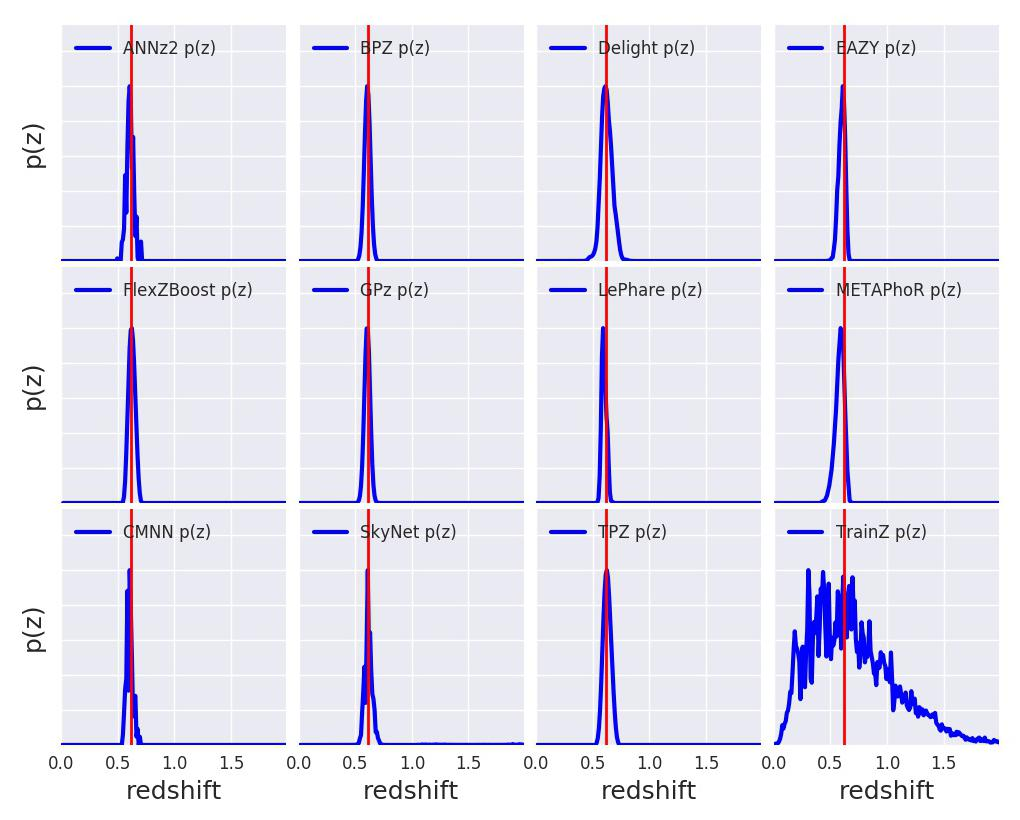
\includegraphics[width=\textwidth]{figures/pz_12codes_261931_crop.jpg}
\end{subfigure}
\begin{subfigure}[b]{0.49\textwidth}
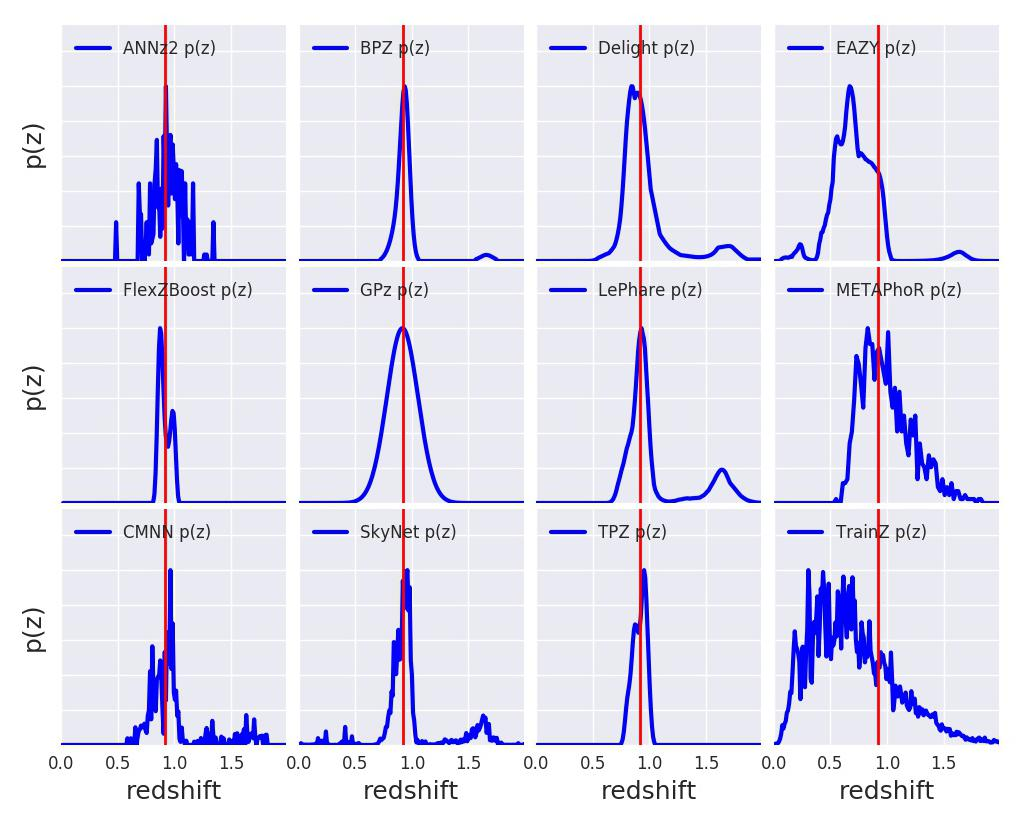
\includegraphics[width=\textwidth]{figures/pz_12codes_471167_crop.jpg}
\end{subfigure}
\begin{subfigure}[b]{0.49\textwidth}
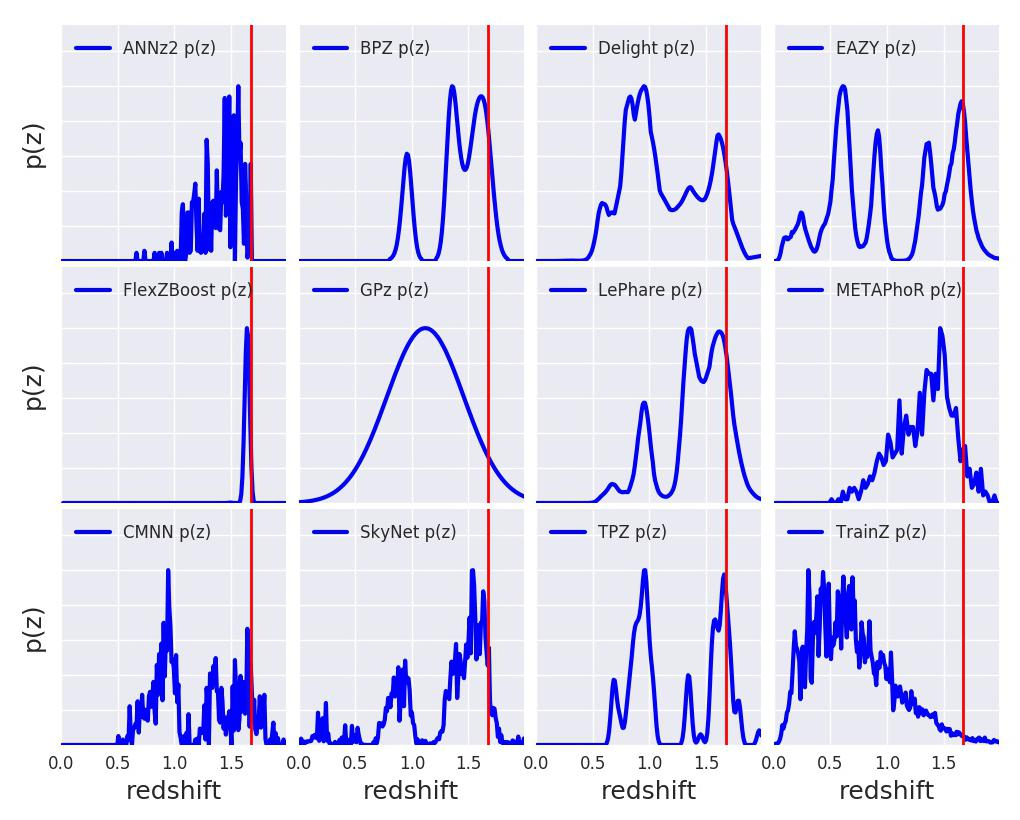
\includegraphics[width=\textwidth]
{figures/pz_12codes_713178_crop.jpg}
\end{subfigure}
\begin{subfigure}[b]{0.49\textwidth}
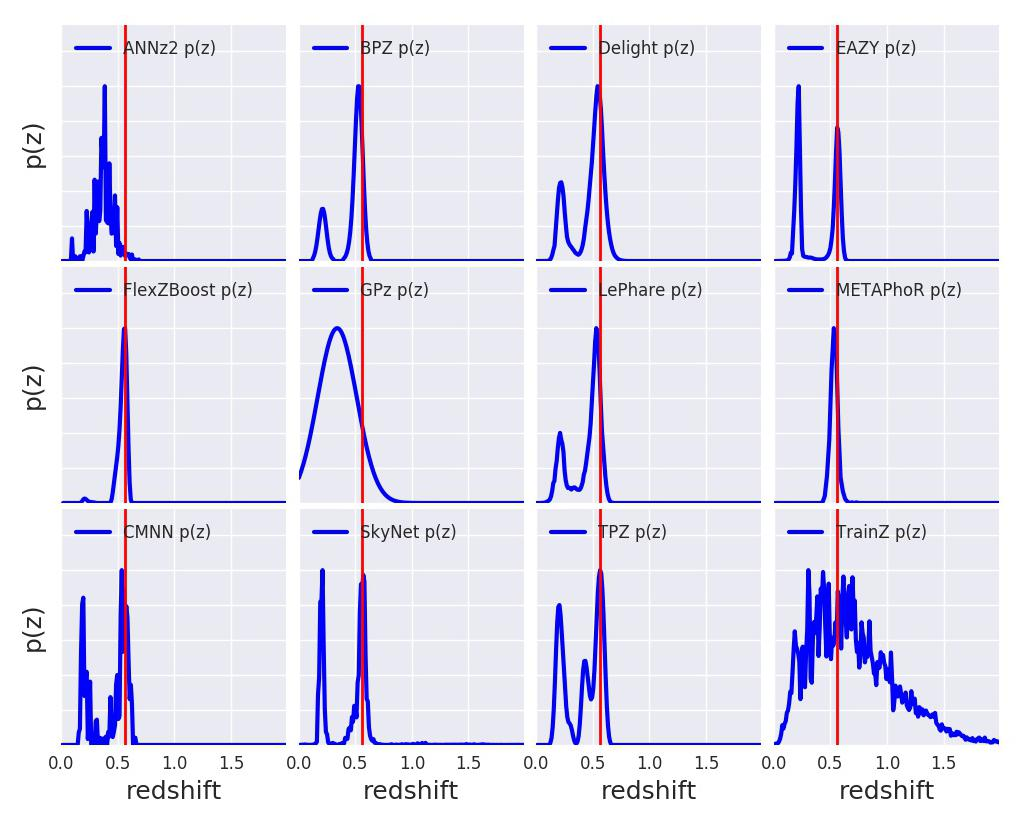
\includegraphics[width=\textwidth]{figures/pz_12codes_982747_crop.jpg}
\end{subfigure}
\caption{Four illustrative examples of individual p(z) distributions produced by the codes.  The red vertical line represents the true redshift.  Examples are chosen with common features seen in PDFs: tight unimodal $p(z)$ (upper left), broad unimodal $p(z)$ (upper right), bimodal $p(z)$ (lower right), and complex/multimodal $p(z)$ (lower left).  Codes show varying amounts of small-scale structure in their reconstruction of the posterior distribution.  We see varying responses from the codes in the presence of color degeneracies and photometric errors, resulting in narrow and broad unimodal, bimodal, and multi-modal $p(z)$ curves.} \label{fig:pz_examples}
\end{figure*}

%\begin{figure*}
%\centering
%\includegraphics[width=\textwidth]{figures/QQplot_11codes.jpg}
%\caption{The QQ plots produced for every photo-$z$ code.  \aim{Consider making this a plot of QQ minus that diagonal for better contrast between methods.}\red{The PIT histogram is essentially this, which is one of the main reasons to include both.  QQ is a fairly standard form, so plotting in this fashion rather than the difference seems better to me, given that we also ahve the PIT histograms. --SJS}} \label{fig:qq}
%\end{figure*}

\begin{figure*}
\centering
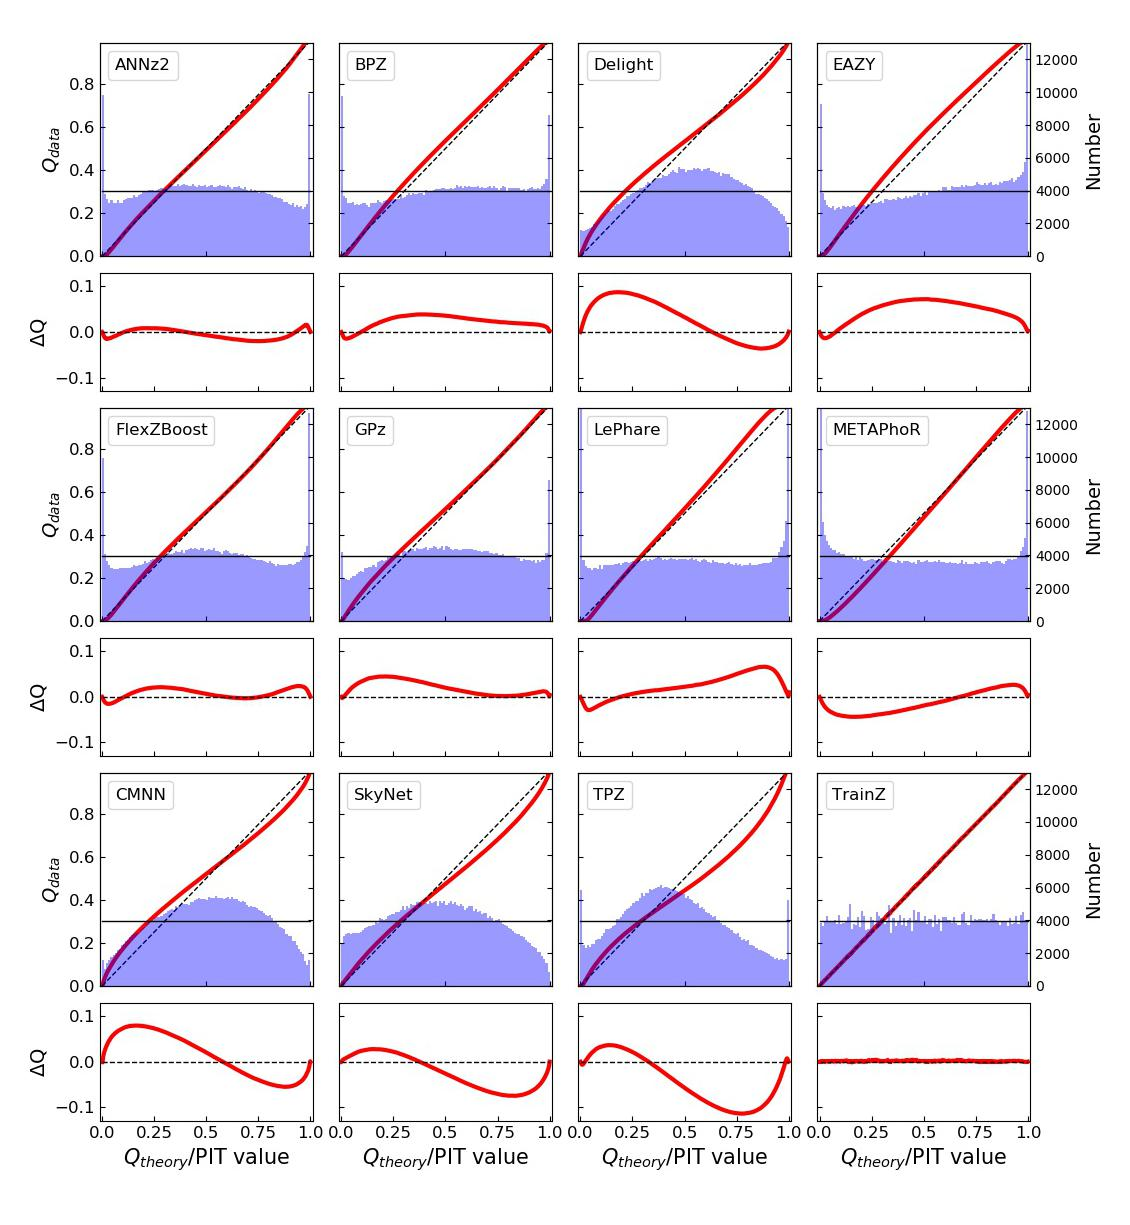
\includegraphics[width=\textwidth]{figures/PITANDQQplot_12codes_crop.jpg}
\caption{Summary plots for all eleven photo-$z$ codes illustrating performance for the interim posterior statistics. The top panel of each pair shows both the Quantile-Quantile (QQ) plot (red) and the histogram of PIT values (blue).  The desired behavior is a QQ plot that matches the diagonal dashed line, and a PIT histogram that matches a uniform distribution matching the thin horizontal black line.  The bottom panel of each pair shows the difference between the QQ quantile and the diagonal, illustrating departure from the desired performance.  Histograms with an overabundance of PIT values at the centre of the distribution indicate $p(z)$ distributions that are overly broad, while an excess of values at the extrema indicate $p(z)$ distributions that are overly narrow.  Values of PIT=0 and PIT=1 indicate ``catastrophic failures'' where the true redshift is completely outside the support of $p(z)$.  Asymmetric features are indicative of systematic bias in the redshift predictions.  A variety of behaviors are evident, and specific details are discussed in the text.}
\label{fig:pitqq}
\end{figure*}

Fig.~\ref{fig:pz_examples} Shows the $p(z)$ produced by each of our eleven photo-$z$ codes for four example galaxies which exemplify some prominent cases that arise when estimating photo-$z$ PDFs: a narrow, unimodal redshift solution, a broader unimodal solution, a bimodal distribution, and a complex, multimodal distribution.   
The red vertical line represents the true redshift of the individual galaxy, and the blue curve represents the redshift probability.  
Several features are obvious even in these illustrative examples.  
\textsc{ANNz2, METAPhoR, NN,} and \textsc{SkyNet} all show an excess of small-scale features, which appear to be print-through of the underlying training set galaxies.  
\textsc{GPZ} (in its current implementation), on the other hand, always produces a single Gaussian, which broadens to cover the multi-modal redshift solutions seen in other codes.

As stated in Section~\ref{sec:metrics}, $p(z)$ is parameterized as $\approx 200$ piecewise constant bins covering $0<z<2$ for all eleven codes, giving a grid size of roughly $\delta z = 0.01$ for each code.  
A piecewise constant grid was a natural choice for some photo-$z$ codes, for instance most template-based codes compute likelihoods on a fixed grid.  
In contrast, FlexZBoost, for example, can return estimates on any grid without compression errors as it’s a basis expansion method where only the expansion coefficients need to be stored.
Codes with a native output format other than the shared piecewise constant binning scheme (or one that can be losslessly converted to it) may suffer from loss of information when converting to it, which could artificially favor some codes over others.

Furthermore, the fidelity of photo-$z$ interim posteriors in this format varies with the quality of the photometry.  
For faint galaxies, this redshift resolution is sufficient to capture the shape of $p(z)$ for the majority of the test sample, where photometric errors on the faint galaxies lead to somewhat broad peaks in the redshift posterior.  
However, as can be seen in e.~g.~the top left panel of Fig.~\ref{fig:pz_examples}, for bright galaxies with narrow $p(z)$ the grid spacing of $\delta z = 0.01$ is not sufficient to resolve the peak.  
This is consistent with the results described in \citet[]{Malz:qp}, who find that quantiles (and, to a lesser degree, samples) often outperform gridded $p(z)$, particularly for bright objects and in the presence of harsher storage constraints.  
With a full 200 numbers to capture the information of each photo-$z$ PDF, any parametrization will perform adequately, but other storage parametrizations and limits on storage resources may be considered in future work.  
%Switching to a quantile based parameterization may be more costly computationally, for example template-based codes would need to test more grid point in order to resolve the quantiles for bright galaxies.  However, the computational time for template based codes scales roughly linearly with the number of grid points, so this may be a reasonable thing to implement.  
We will discuss this further in Section~\ref{sec:discussion}.
% \red{someone review this statement to make sure that I'm saying this correctly!}

Fig.~\ref{fig:pitqq} shows both the quantile-quantile plots (red) and the histogram of PIT values (blue) summarizing the results from each photo-$z$ code.  The red line shows the measured quantiles, while the black diagonal represents the ideal QQ values if the distribution were perfectly reproduced.  A second panel below the main panel for each code shows the difference between $Q_{data}$ and $Q_{theory}$, i.~e.~the departure from the diagonal, for clarity.
Biases and trends in whether the average width of the $p(z)$ values being over/under-predicted are evident.  An overall bias where the predicted redshift is systematically low manifests as the measured QQ value falling above the diagonal, as is the case for \textsc{BPZ} and \textsc{EAZY}, while a systematic overprediction shows up as the measured QQ value falling below the diagonal, as seen in \textsc{TPZ}.  In terms of PIT histograms, a systematic underprediction of redshift corresponds to fewer PIT values at $PIT<0.5$ and more at $PIT>0.5$, while a systematic overprediction will show the opposite.

Examination of the PIT histograms and QQ plots shows that there are fairly generic issues with the width of $p(z)$ uncertainties: \textsc{Delight, NN, SkyNet} and \textsc{TPZ} all show a PIT histogram with an dearth of low values and and an excess of high values, signs that, on average, their $p(z)$ are more broad than the true distribution of redshifts.  \textsc{METAPhoR} shows the opposite trend, indicating the the $p(z)$  are more narrow than the distributions given by the true redshifts.  In all of these code cases there is a free parameter or bandwidth that can be used to tune uncertainties.  The sensitivity of multiple codes to this bandwidth choice emphasizes the fact that great care must be taken in setting user-defined parameters in photo-$z$ codes, even in the presence of representative training/validation data.  for \textsc{FlexZBoost} the ``sharpening'' parameter (described in Section~\ref{sec:flexzboost}) plays a key role in improving the results, resulting in a QQ plot that is very nearly diagonal.  A similar sharpening procedure could be beneficial for several codes.
Interestingly, the three purely template-based codes, \textsc{BPZ, EAZY}, and \textsc{LePhare}, show relatively well behaved $p(z)$ statistics (albeit with some bias), which may indicate that the likelihood estimation with representative templates is accurately capturing the uncertainties on individual redshifts. 

%Fig.~\ref{fig:pitqq} shows the PIT histogram plots produced by each photo-$z$ code. 
%These plots show information that is very similar to that shown in the QQ plot in many ways. 
The ideal PIT histogram would follow the black dashed line, representing a uniform distribution of PIT values, equivalent to the diagonal line in the QQ plot.
Overly broad $p(z)$ values show up as an excess of PIT values near $0.5$ and a dearth of values at the edges, while overly narrow $p(z)$ will have an excess at the edges and will be missing values at the centre.
Another feature evident in the PIT histograms is the number of ``catastrophic outlier'' values where the true redshift falls outside of the non-zero support of $p(z)$, corresponding to PIT$=0.0$ or $1.0$ is more apparent than in the QQ plots.  Following Kodra \& Newman (in prep.) we define $f_{\rm O}$ as the fraction of objects with $PIT<0.0001$ or $PIT>0.9999$.  Table~\ref{tab:pitoutlier} lists these fractions for each of the codes. For a proper Uniform distribution we expect a value of $0.0002$.  Several codes show a marked excess, with \textsc{ANNz2, FlexZBoost, LePhare, and METAPhoR} with $f_{\rm O} > 0.02$, indicating a sizeable number of catastrophic redshift solutions where the true redshift is not covered by the extent of $p(z)$.  For \textsc{METAPhoR} this may be partially due to an overall underprediction of the $p(z)$ width, however this is not the case for the other codes.  \textsc{LePhare} is a particular outlier with nearly 5 per cent of objects outside of $p(z)$ support.  Further study will be necessary to determine what is causing these misclassifications for \textsc{LePhare}.  As expected, and by design, \textsc{TrainZ} has the proper fraction of outliers for the $f_{\rm O}$ statistic.


\begin{table}
\setlength{\tabcolsep}{2pt}
\centering
\caption{The fraction of ``catastrophic outlier'' PIT values.  We expect a value of 0.0002 for a proper Uniform distribution.  An excess over this small value indicates true redshifts that fall outside the non-zero support of the $p(z)$.  }\label{tab:pitoutlier}
\begin{tabular}{lc}
\hline
\hline
 ``catastrophic outlier''\\ PIT fraction\\
\hline
Photo-z Code & fraction PIT$<10^{-4}$ or $>$0.9999\\
\hline
\textsc{ANNz2} & 0.0265\\
\textsc{BPZ} & 0.0192\\
\textsc{Delight} & 0.0006\\
\textsc{EAZY} & 0.0154\\ 
\textsc{FlexZBoost} & 0.0202\\
\textsc{GPz} & 0.0068\\ 
\textsc{LePhare} & 0.0486\\
\textsc{METAPhoR}& 0.0229\\
\textsc{CMNN} & 0.0034\\ 
\textsc{Skynet} & 0.0001\\  
\textsc{TPZ} & 0.0130\\
\hline
\textsc{TrainZ} & 0.0002\\
\end{tabular}
\end{table}


%\begin{figure*}
%\centering
%\includegraphics[width=\textwidth]{figures/PIT_histogram_plot_11codes.jpg}
%\caption{The PIT histogram plots produced for every photo-$z$ code.  Ideal behaviour would match a uniform distribution, indicated by the horizontal dashed line.  Histograms with an overabundance of PIT values at the centre of the distribution indicate $p(z)$ distributions that are overly broad, while an excess of values at the extrema indicate $p(z)$ distributions that are overly narrow.  Values of PIT=0 and PIT=1 indicate ``catastrophic failures'' where the true redshift is completely outside the support of $p(z)$.  Asymmetric features are indicative of systematic bias in the redshift predictions.
%\aim{Could we combine this with the previous figure by plotting both as differences from ideal on one plot with left and right axis labels?  The information seems degenerate (which makes sense!)}\red{as you say, the information is degenerat, this form emphasizes the differences a bit more, and shows off the catastrophic outliers with PIT=0 and 1 a bit better in my mind.} } \label{fig:pit}
%\end{figure*}
\begin{figure*}
\centering
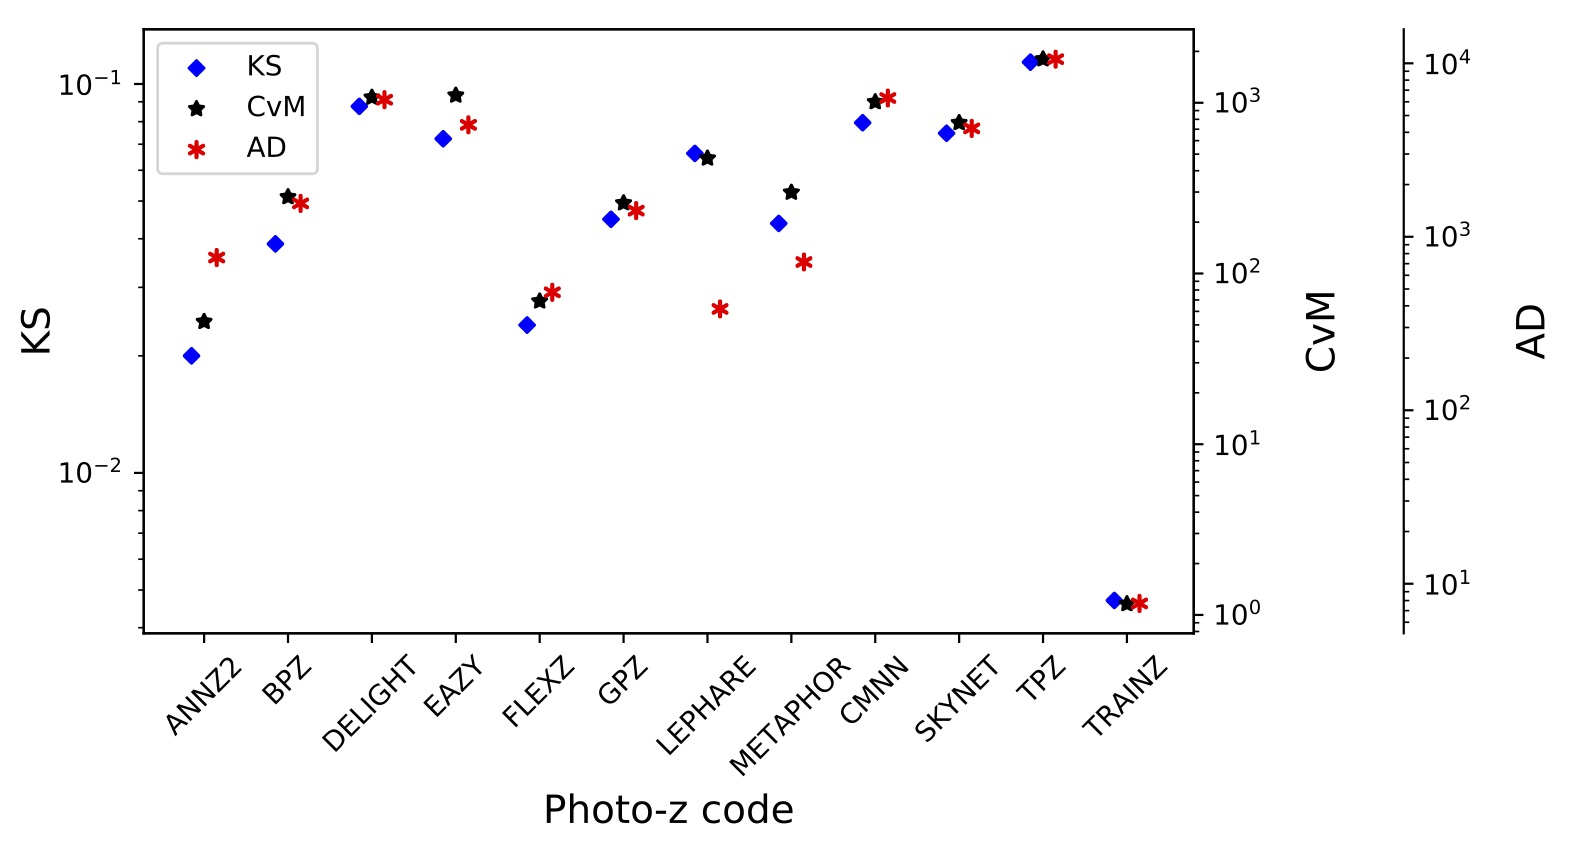
\includegraphics[width=\textwidth]{figures/KSvsCvMvsAD_PIT_withnull_jpg.jpg}
\caption{A visual representation of the Kolmogorov-Smirnoff (KS, blue diamond), Cramer-von Mises (CvM, black star), and Anderson-Darling (AD, red asterisk) statistics for the PIT distributions.  The statistics are often highly correlated, though the AD statistic truncates the extrema of the distribution and can have disparate values compared to KS and CvM.} \label{fig:pit_stats}
\end{figure*}

Fig.~\ref{fig:pit_stats} shows comparative metric values for the quantitative Kolmogorov-Smirnoff (KS), Cramer-Von Mises (CvM), and Anderson Darling (AD) test statistics for each of the codes based on comparing the distribution of their PIT values to the expected uniform distribution over the interval [0,1].  The individual values of the statistic are not as important as the comparative score between the different codes.   
%\red{Can p-values be supplied for each statistic? The statistics themselves are difficult to interpret, other than ``lower is better'' (p-value in skgof was broken, having trouble finding 1-sample KS calculation for uniform distribution)}
The AD test statistic diverges for values that include the extrema, and thus is calculated by excluding the edges of the distribution.  
We calculate the AD statistic over the range of PIT values $v=[0.01,0.99]$.  \textsc{ANNz2} and \textsc{FlexZBoost} score very well for the PIT metrics.  
\textsc{METAPhoR} and \textsc{LePhare} score very well in the PIT AD statistic, but both have a large number of catastrophic outliers, resulting in higher KS and CvM scores.

Given the near-perfect training data, examining the individual codes for explanations for departures from the expected behaviour will be instructive in avoiding similar problems in future tests. 
\textsc{ANNz2} performs quite well in $p(z)$ based metrics.  In the specific implementation employed in this paper, the final $p(z)$ is a weighted average of five neural-nets.  During the training process \textsc{ANNz2} compares the percentiles of the redshift training sample against the CDFs of the $p(z)$ sample.  Distributions that more closely match are given extra weight, and the final weights are designed to produce accurate percentiles.  Given that our metrics are focused on the percentile distributions, it is unsurprising that \textsc{ANNz2} performs well in the given metrics.  The discreteness in the individual $p(z)$ estimated by \textsc{ANNz2} can be attributed to the fact that the code was run as a classifier, assigning weights to discrete bins of redshift.  While multiple bins may receive weight, the bins themselves will still be discretized, and no additional smoothing was performed.
Overall, \textsc{FlexZBoost} and \textsc{ANNz2} show the best ensemble agreement in their distribution of PIT values.

\subsection{Metrics of the stacked estimator of the redshift distribution}\label{sec:stackedmetrics}

\begin{figure*}
\centering
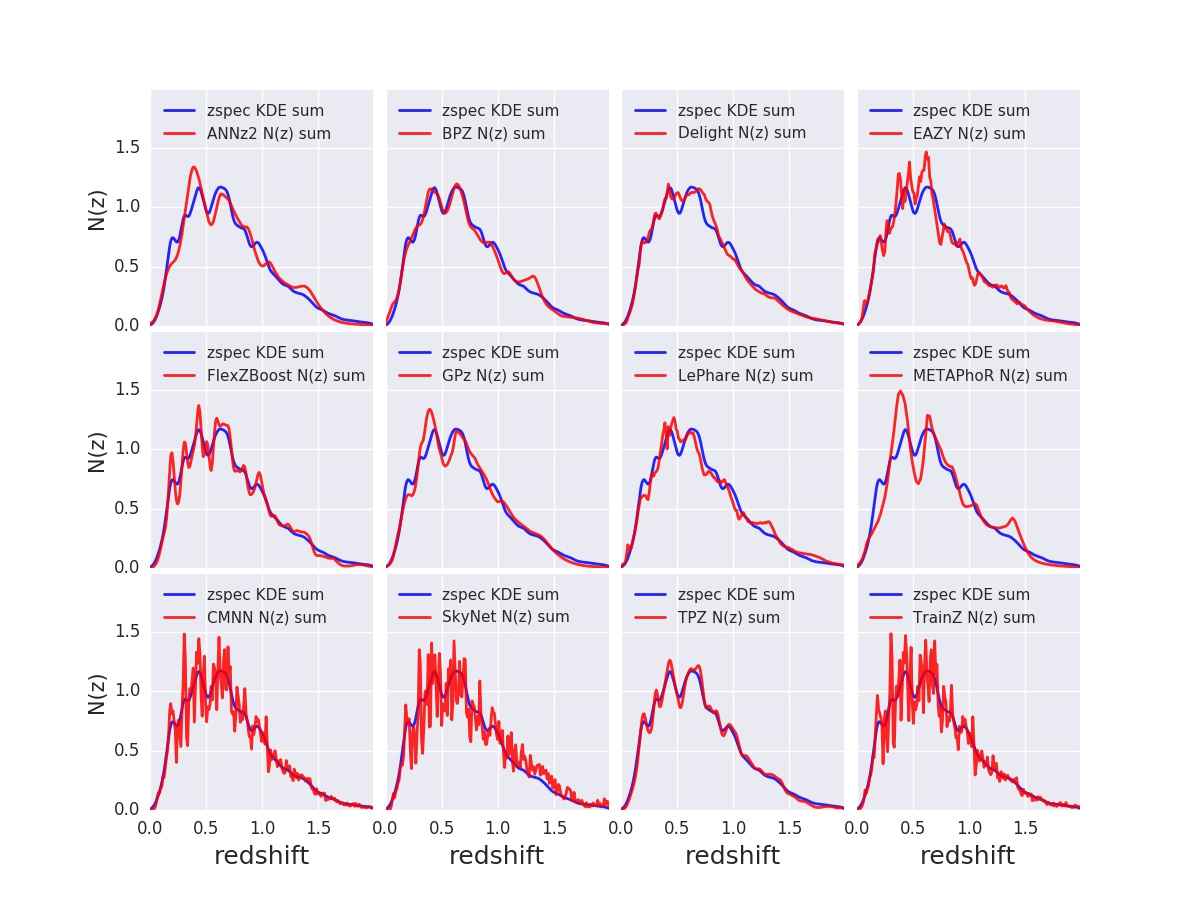
\includegraphics[width=\textwidth]{figures/NZsumplot_12codes.jpg}
\caption{The stacked $p(z)$ produced by each photo-$z$ code ($\hat{N}(z)$, red) compared to the spectroscopic redshift distribution ($N'(z)$, blue).  Varying levels of small-scale structure are seen in the codes.  $N'(z)$ is smoothed using a single bandwidth chosen via Scott's rule for all codes.} \label{fig:nz}
%\aim{Arguably this could also be clarified by showing the true $n'(z)$ once and then differences from it for each cod's stacked estimator\dots}\scc{what if we plot the difference between true and stacked rather than soverposing the two lines? Sam please do not hate me.}
\end{figure*}

\begin{figure*}
\centering
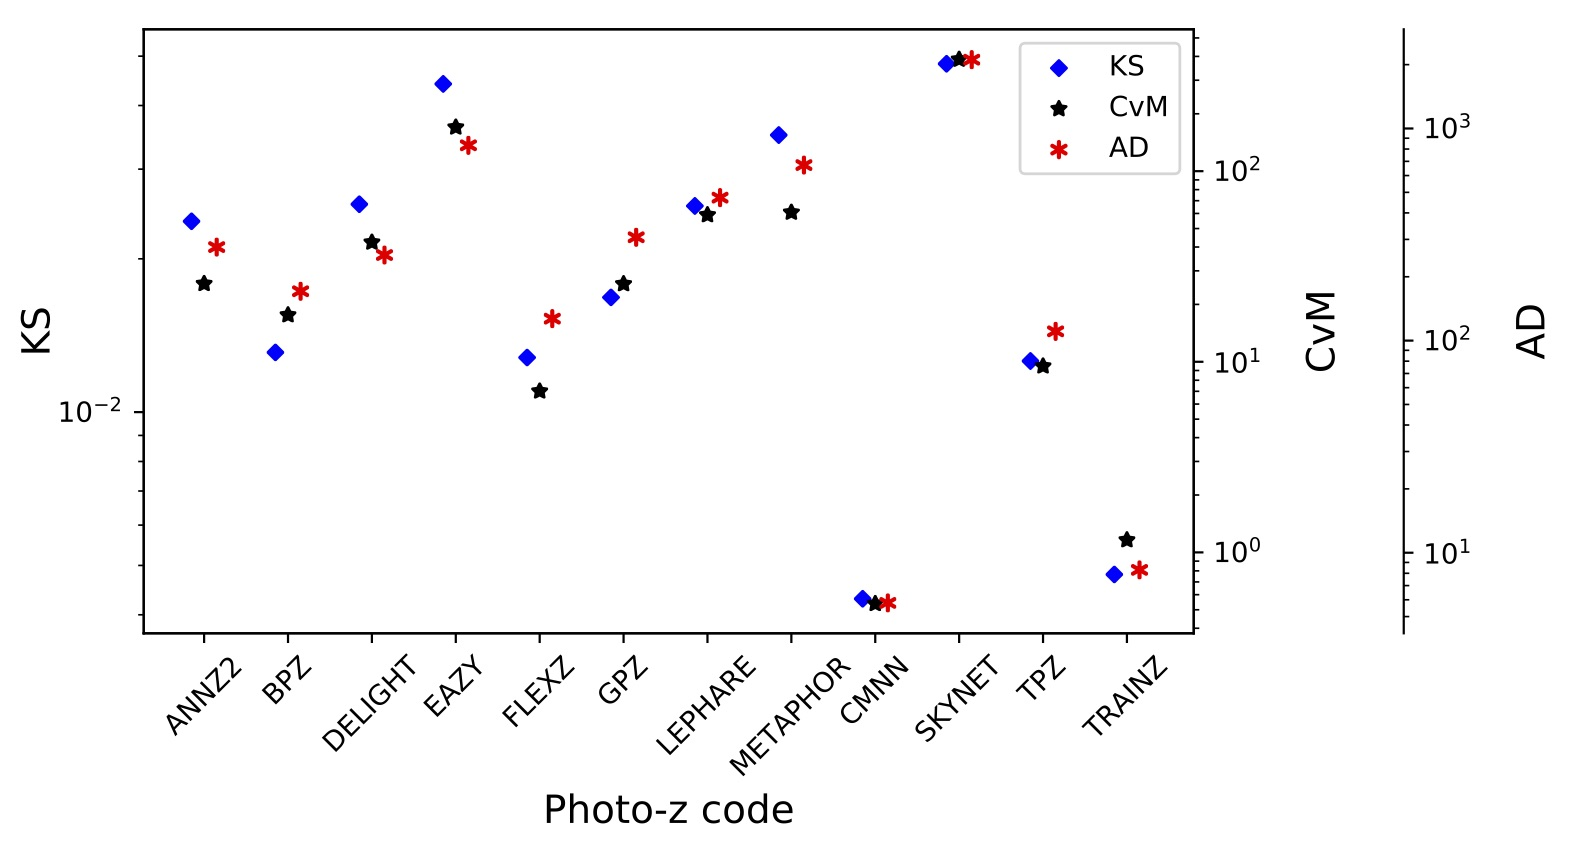
\includegraphics[width=\textwidth]{figures/KSvsCvMvsAD_NZ_withnull_jpg.jpg}
\caption{A visual representation of the Kolmogorov-Smirnoff (KS, blue diamond), Cramer-von Mises (CvM, black star), and Anderson-Darling (AD, red asterisk) statistics for the $\hat{N}(z)$ distributions. The statistics are correlated, the codes with the lowest KS statistics tend to have the lowest CvM and AD statistics.  \textsc{CMNN} performs markedly better than the others in reconstructing the overall $N(z)$ distribution, while \textsc{SkyNet} scores poorly due to an overall bias in its redshift predictions.} \label{fig:nz_stats}
\end{figure*}

Fig.~\ref{fig:nz} shows the stacked $\hat{N}(z)$ distribution compared to the true redshift distribution $N'(z)$ for all tested codes.  The red line indicates the summed $p(z)$ for each code, while the blue line shows the true redshift distribution smoothed via kernel density estimation (KDE), with a bandwidth chosen via Scott's rule \citep{Scott:1992}.  While Scott's rule is used to display $N'(z)$ in the figure, all quantitative statistics are computed via the empirical CDF, and are thus unaffected by bandwidth/smoothing choice.  
Several of the codes show an excess at $z \sim 1.4$, particularly the template-based codes \textsc{BPZ}, \textsc{EAZY}, and \textsc{LePhare}.  
This is likely due to the $4000$ angstrom break passing through the gap between the $z$ and $y$ filters.  
This feature is one of the most prominent in individual galaxy p(z), and is readily seen in the point-estimate plots shown in Fig.~\ref{fig:pz_pointestimates} and described in the Appendix.  
Several of the machine learning based codes appear to be over-trained, adding excess galaxy probability to the redshift peaks and missing probability in the troughs.  
Given that our training data is drawn from the same galaxy population as the test set, and our data has prominent peaks in $N'(z)$, perhaps it is not unexpected that such overtraining occurs. 
A more extensive training/validation set might allow for a better choice of smoothing parameters in individual codes that would avoid such overtraining.

%\aim{Move the text on Scott's Rule to Discussion?}
%Scott's rule \citep{Scott:1992} was used to determine the smoothing bandwidth of the true redshift sample: that is, a single smoothing scale was chosen to represent the true redshift sample for all eleven codes.  

As with the $p(z)$ values in Figure~\ref{fig:pitqq}, different levels of substructure are obvious for the different codes.  
While Scott's rule provides a relatively good general smoothing scale to represent the true $N'(z)$, there are smaller scale fluctuations: while \textsc{FlexZBoost} and \textsc{CMNN} appear somewhat discrepant in Fig.~\ref{fig:nz}, they are actually the two most accurate in terms of their quantitative measurements.   
%\textsc{SkyNet} also shows excess small-scale structure, but also shows significant overestimate of the high redshift galaxy population.  
Interestingly, while \textsc{ANNz2} shows an abundance of small scale structure in individual $p(z)$ measurements (see Fig.~\ref{fig:pz_examples}), the summed $\hat{N}(z)$ is rather smooth, where the small scale features average out.  This is not the case for the two other codes that show an abundance of substructure in their individual $p(z)$: both \textsc{CMNN} and \textsc{SkyNet} show small scale features both in $p(z)$ and $\hat{N}(z)$.  For \textsc{CMNN} the $p(z)$ are a simply a weighted histogram of all spectroscopic training galaxies in nearby colour space with no smoothing applied, so the substructure is not unexpected.  The PIT histogram and shape of the QQ plot in Figure~\ref{fig:pitqq} show that \textsc{CMNN} is producing $p(z)$ that are overly broad, additional smoothing of the $p(z)$ would exacerbate this problem.  While the $\hat{N}(z)$ plot shows more small scale features than other codes, these features are actually representative of real structure in the true $N'(z)$, as evidenced by the very good metric scores for \textsc{CMNN}.  \textsc{SkyNet} $p(z)$ were also not smoothed: while previous implementations of the code such as \citet{Sanchez:14} and \citet{Bonnett:15} (see Appendix C.3) implement a ``sliding bin'' smoothing, no such procedure was used in this study.  In addition to excess substructure, \textsc{SkyNet} shows an obvious redshift bias, evident both visually in Figure~\ref{fig:nz} and in the first moment of N(z) listed in Table~\ref{tab:moments}, where it is clearly an outlier.  \textsc{SkyNet} employed a method where a random sample of training galaxies was chosen, but there was no test that the subset was completely representative of the overall redshift distribution.  Also unlike \citet{Bonnett:15}, no effort was made to add extra weight to more rare low and high redshift galaxies.  Either of these decisions could be the cause of the bias seen in our results.  Future runs of \textsc{SkyNet} will explore these implementation choices and their effects.


Figure~\ref{fig:nz_stats} shows the quantitative Kolmogorov-Smirnoff (KS), Cramer-Von Mises (CvM), and Anderson Darling (AD) test statistics for each of the codes for the $\hat{N}(z)$ based measures.
%\red{Can p-values be supplied for each statistic? The statistics themselves are difficult to interpret, other than ``lower is better'' (no, p-values are very difficult to compute for non-uniform distributions)}
\textsc{FlexZBoost}, \textsc{CMNN}, and \textsc{TPZ} outperform the other codes in the $\hat{N}(z)$ metrics.  
It is unsurprising that \textsc{CMNN} scores well, as with a near perfectly representative training set means that choosing neighbouring points in color/magnitude space should lead to excellent agreement in the final $\hat{N}(z)$ estimate.  \textsc{TPZ} performed quite poorly in $p(z)$ statistics, but results in a good fit to the overall $N(z)$.  This is somewhat surprising, as performance was optimized for accurate $p(z)$, not $\hat{N}(z)$.  During the validation stage for \textsc{TPZ}, there was a trade off between the width of the $p(z)$ when adjusting a smoothing parameter and overall redshift bias.  The optimal result in the PIT metrics, as illustrated in the shape of the QQ plot, does contain some level of bias as well as a slight underprediction of mean $p(z)$ width, which translates to poor metric scores.  This is something that will be looked into for \textsc{TPZ} in the future.

It is also of note that all three template-based codes show an excess in their stacked $p(z)$ at $z\,\sim\,1.3-1.4$.  This redshift range corresponds to the wavelengths where the $4000$ Angstrom break is passing between the borders of the $z$ and $y$ filters.  This strong break entering the gap between the two reddest filters can cause problems with redshift estimation of individual galaxies, as can be seen in the point-estimate photo-$z$'s shown in Figure~\ref{fig:pz_pointestimates}.  This is not unique to this dataset, it is a common occurrence in photo-$z$ estimation.  The fact that similar excesses appear in Figure~\ref{fig:nz} for \textsc{ANNz2} and \textsc{METAPhoR} shows that the effect is not limited to template-based codes.  However, the lack of such a feature in the other codes shows that it is possible to eliminate the degeneracies.  Further study on this issue may provide a solution for codes that suffer from this shortcoming.


%\red{discussion of why NN and FZBoost are doing well, how we can try to improve the other codes} 
%\textcolor{cyan}{Ann: }


Table~\ref{tab:cdeloss} shows the CDE loss statistic for each photo-$z$ code.  Once again \textsc{FlexZBoost} and \textsc{CMNN} score very well for the stacked $\hat{N}(z)$ metrics, as do \textsc{GPz} and \textsc{TPZ}.  The CDE loss measures how well individual PDFs are estimated, and codes with a low CDE loss tend to have good $\hat{N}(z)$ estimates (though the reverse is not necessarily true). \textsc{FlexZBoost} is optimized to minimize CDE loss which may explain why the method has good ensemble metrics as well. Note from Table~\ref{tab:cdeloss} that both \textsc{FlexZBoost} and \textsc{CMNN} have low CDE losses.  Empirically, we have found that PIT RMSE is not as closely correlated to CDE loss as it is to the $N(z)$ statistics.  As CDE loss is a better measure of individual redshift performance, rather than ensemble distribution performance, this statistic is a better indicator of which codes will be most likely to perform well for science cases where single objects are employed.

Table~\ref{tab:rmse} gives the root-mean-square-error (RMSE) statistics for both the PIT and N(z) estimators.  The PIT value calculates the RMSE between the quantiles shown in the QQ plot in Figure~\ref{fig:pitqq} and the diagonal, while the N(z) calculates the RMSE between the cumulative distribution of the stacked $\hat{N}(z)$ and the true redshift distribution $N'(z)$.  %\red{more about RMSE?  Or remove it? It's barely described in Section~\ref{sec:metrics} and wasn't even referred to in the text until I added this on June 29th--SJS.}

Table~\ref{tab:moments} lists the first three moments of the stacked $\hat{N}(z)$ distribution, including the moments of the ``truth'' distribution for comparison.  Several codes are able to reproduce the mean and variance of the distribution to less than a per cent, while several codes do not, which may be a cause for concern, given that mean and variance of the redshift distribution are key properties in cosmological analyses.  We note that this stated goal of the study as defined for participants was to accurately reproduce $p(z)$, the ``stacking'' of the probability distributions to estimate $\hat{N}(z)$ was not the focus as stated to the participants.  This explains why some of the best-performing empirical codes in terms of $p(z)$ measures (e.~g.~\textsc{FlexZBoost}) do not do as well at reproducing $\hat{N}(z)$ moments.  Had we defined a different parameter to optimize, in this case overall accuracy of $\hat{N}(z)$ rather than individual $p(z)$, would result in improved performance in a particular metric.  That is, optimizing photo-$z$ performance for one metric does not automatically give optimal performance for other metrics.  As previously stated, there are a variety of scientific use cases for photo-$z$'s in large upcoming surveys, and care must be taken in how the metrics used to optimize catalog photometric redshifts are defined as well as in how they are used.  In addition, very few scientific use cases will employ the overall $\hat{N}(z)$ with no cuts, as we explore in this paper.  We discuss more realistic tomographic bin selections that will be explored in a follow-up paper in Section~\ref{sec:futurework}.
%\red{[mention that we are calculating moments for the entire sample, will look at fiducial tomographic bins in a follow-up paper (unless group and reviewers realy think we should include in this paper.]}
%\red{FlexZBoost has some of the best $n(z)$ statistics, but the moments are not good.  Why is this?  Is it the over/underprediction of the high redshift part of the distribution?  Discuss this after talking with Rafael.}

%\subsection{Response of Individual Codes}
%\label{sec:res:pz_indiv_codes}
%\red{this may be incorporated in to 5.1 and 5.2 rather than live in its own section!}


%\red{HOW CODES deal with negative fluxes, and magnitude uncertainties}

%\red{overall conclusions of the Results section}

\subsection{Interpretation of metrics}\label{sec:caution}
%Caution on metrics and photo-$z$ codes}\label{sec:caution}
%(Alex Malz, Sam Schmidt)

Samples from accurate photo-$z$ posteriors should reproduce the space of $p(z, data)$. However, it is difficult to test this reconstruction given our data set, as the galaxy distributions arise from mock objects pasted on to an underlying dark matter halo catalogue with properties designed to match empirical relations, rather than being drawn from statistical distributions in redshift.  In previous sections we have mentioned that optimizing for a specific metric does not guarantee good performance on other metrics, nor is there any guarantee that good performance by our metrics corresponds to \textit{accurate} photo-$z$ posteriors.  
%\aim{Explain that samples from accurate photo-$z$ posteriors should reconstruct the space of $p(z, data)$, a test we can't check with our datasets.}  
In other words, we can construct photo-$z$ estimators that provide good coverage in many of our tests, but which have very little predictive power.  


The \trainz\ estimator, which assigns every galaxy a $p(z)$ equal to $N(z)$ of the training set as described in Section~\ref{sec:method:trainz}, is introduced as a ``null test'' to demonstrate this point via \textit{reductio ad absurdum}.  
\trainz\ outperforms all codes on the PIT-based metrics, and all but one code on the $N(z)$ based statistics.  
Because our training set is perfectly representative of the test set, $N(z)$ should be identical for both sets down to statistical noise.
%\textit{Explain the connection between \trainz\ and these metrics.}

The CDE loss and point estimate metrics, however, successfully identify problems with \trainz.  
As shown in Appendix~\ref{sec:pointmetrics}, \trainz has identical $ZPEAK$ and $ZWEIGHT$ values for every galaxy, and thus the photo-$z$s are constant as a function of spec-$z$s, i.e. a horizontal line at the mode and mean of the training set distribution respectively.  The explicit dependence on the \it{individual} posteriors in the calculation of the CDE loss, described in Section~\ref{sec:CDE_loss}, distinguishes this metric from the other $p(z)$ metrics that test the overall ensemble of $p(z)$ distributions.  With a representative training set, \trainz\ will score well on the ensemble metrics, but fails miserably for metrics tied to individual redshifts.  We note that many of the ensemble-based metrics are prominent in the photo-$z$ literature despite their inability to identify problems such as those exemplified by \trainz.

%\aim{Explain why CDE loss is different from other metrics (isn't fooled by \trainz) and note that the others have more of a presence in the literature despite their flaw of failing to identify this severe problem.}

% While looking at one, or even most of our metrics would have given the impression that this estimator was nearly optimal, red flags in CDE loss and point estimates reveal the problems.  
%[more caution on over-reliance on metrics, and making sure that metrics test all of what you want] \red{this definitely still needs work}
In summary, context is crucial to interpreting metrics and defending against the likes of \trainz.
The best photo-$z$ method is the one that most effectively achieves our science goals, not the one that performs best on a metric that does not accurately reflect those goals.
In the absence of clear goals or the information necessary for a principled metric definition, we must think carefully before choosing a single metric

%\begin{table*}  %%% DATA TABLE %%%
%\caption{KS, CvM and AD statistics for each photo-$z$ code.} \label{tab:results}
%PIT statistic
%
%\begin{tabular}{lrrrr}
%\hline
%\bf Photo-$z$ Code & \bf KS & \bf CvM & \bf AD & \bf AD \\
%                   &        &         & $v=[0.05,0.95]$ & $v=[0.01,0.99]$        \\
%\hline
%\textsc{ANNz2} 		& $0.0200$ &   $52.25$ &   $583.0$ &   $759.2$ \\
%\textsc{BPZ} 		& $0.0388$ &  $280.79$ &  $1361.4$ &  $1557.5$ \\
%%\textsc{Delight} 	& $0.1380$ & $3040.59$ & $13880.2$ & $17761.4$ \\
%\textsc{Delight}    & $0.0876$ & $1075.17$ & $4407.8$  & $6167.5$\\
%%\textsc{EAZY} 		& $0.0690$ &  $994.19$ &  $3479.5$ &  $4158.8$ \\
%\textsc{EAZY}       & $0.0723$ & $1105.58$ & $3475.0$  & $4418.6$\\
%%\textsc{FlexZBoost} & $0.0260$ &   $70.58$ &   $595.0$ &   $533.0$ \\
%\textsc{FlexZBoost} & $0.0240$ &   $68.83$ &   $567.9$ &   $478.8$\\
%\textsc{GPz} 		& $0.0449$ &  $258.56$ &   $904.8$ &  $1414.8$ \\
%\textsc{LePhare} 	& $0.0663$ &  $473.05$ &    $85.9$ &   $383.8$ \\
%\textsc{METAPhoR} 	& $0.0438$ &  $298.56$ &   $248.6$ &   $715.5$ \\
%%\textsc{CMNN} 		& $-$ & $-$ & $-$ & $-$ \\
%\textsc{CMNN}         & $0.0795$  &$1011.11$ &  $3908.2$ &  $6307.5$ \\
%\textsc{SkyNet} 	& $0.0747$ &  $763.00$ &  $2740.2$ &  $4216.4$ \\
%\textsc{TPZ} 		& $0.1138$ & $1801.74$ &  $9046.2$ & $10565.7$ \\
%%\textsc{Frankenz}	& $-$ & $-$ & $-$ & $-$ \\
%\hline
%\end{tabular}

%Stacked $n(z)$ statistic
%
%\begin{tabular}{lrrrr}
%\hline
%\bf Photo-$z$ Code & \bf KS & \bf CvM & \bf AD & \bf AD \\
%                   &        &         & $z=[0.002,2.0]$ & $z=[0.0,2.0]$        \\
%\hline
%\textsc{ANNz2} 		& $0.0237$ &  $25.676$ &   $276.4$ &   $276.0$ \\
%\textsc{BPZ} 		& $0.0131$ &  $17.587$ &   $169.0$ &   $170.9$ \\
%%\textsc{Delight} 	& $0.0184$ &  $18.975$ &   $151.5$ &   $151.5$ \\
%\textsc{Delight}    & $0.0256$ &  $42.341$ &   $253.3$ &   $253.2$ \\
%%\textsc{EAZY} 		& $0.0434$ & $167.329$ &   $811.3$ &   $817.0$ \\
%\textsc{EAZY}       & $0.0441$ & $169.977$ &   $827.7$ &   $833.3$ \\
%%\textsc{FlexZBoost} & $0.0065$ &   $2.764$ &    $24.7$ &    $24.6$ \\
%\textsc{FlexZBoost} & $0.0128$ &   $7.007$ &  $127.02$ &   $126.9$\\
%\textsc{GPz} 		& $0.0168$ &  $25.605$ &   $307.1$ &   $307.1$ \\
%\textsc{LePhare} 	& $0.0254$ &  $58.900$ &   $477.4$ &   $472.0$ \\
%\textsc{METAPhoR} 	& $0.0350$ &  $60.790$ &   $671.9$ &   $672.3$ \\
%%\textsc{CMNN} 		& $-$ & $-$ & $-$ & $-$ \\
%\textsc{CMNN}         & $0.0043$ & $0.538$   &   $5.6$   &      $5.8$ \\
%\textsc{SkyNet} 	& $0.0483$ & $385.830$ &  $2119.4$ &  $2110.3$ \\
%\textsc{TPZ} 		& $0.0126$ &   $9.483$ &   $110.7$ &   $110.6$ \\
%%\textsc{Frankenz}	& $-$ & $-$ & $-$ & $-$ \\
%\hline
%\end{tabular}
%\end{table*}

\begin{table}  %%% DATA TABLE %%%
\centering
\caption{CDE loss statistic for each photo-$z$ code.} \label{tab:cdeloss}
\begin{tabular}{lr}
\hline
\bf Photo-$z$ Code & \bf CDE Loss \\
\hline
\textsc{ANNz2} 		& $-6.88$ \\
\textsc{BPZ} 		& $-7.82$ \\
%\textsc{Delight} 	& $-4.06$ \\
\textsc{Delight}    & $-8.33$\\
%\textsc{EAZY} 		& $-7.97$ \\
\textsc{EAZY}       & $-7.07$ \\
%\textsc{FlexZBoost} & $-11.51$ \\
\textsc{FlexZBoost} & $-10.60$\\
\textsc{GPz} 		& $-9.56$ \\
\textsc{LePhare} 	& $-1.66$ \\
\textsc{METAPhoR} 	& $-6.28$ \\
%\textsc{CMNN} 		& $-$ \\
\textsc{CMNN}         & $-10.43$ \\
\textsc{SkyNet} 	& $-7.89$ \\
\textsc{TPZ} 		& $-9.55$ \\
\hline
\trainz		& $-0.83$ \\
%\textsc{Frankenz}	& $-$  \\
%\hline
\end{tabular}
\end{table}

\begin{table}
\setlength{\tabcolsep}{2pt}
\begin{center}
\caption{Root-Mean-Square-Error (RMSE) statistics for the eleven photo-z codes for both PIT and $\hat{N}(z)$ distributions.}\label{tab:rmse}
\begin{tabular}{lcc}
\hline
\hline
Root-Mean-Square-Error \\
(RMSE) statistics \\
\hline
Photo-z Code & PIT RMSE & N(z) RMSE\\
\hline
\textsc{ANNz2}      & 0.019 & 0.0054\\
\textsc{BPZ}        & 0.032 & 0.0050\\
\textsc{Delight}    & 0.111 & 0.0056\\
\textsc{EAZY}       & 0.054 & 0.0102\\
\textsc{FlexZBoost} & 0.021 & 0.0022\\
\textsc{GPz}        & 0.048 & 0.0042\\
\textsc{LePhare}    & 0.028 & 0.0062\\
\textsc{METAPhoR}   & 0.064 & 0.0081\\
\textsc{CMNN}         & 0.108 & 0.0009\\
\textsc{Skynet}     & 0.054 & 0.0144\\ 
\textsc{TPZ}        & 0.082 & 0.0031\\
\hline
\trainz		& 0.0025 & 0.0013\\
\end{tabular}
\end{center} 
\end{table}

%\begin{table}
%\begin{center}
%caption{RMSE Statistics for the 11 Photo-z codes for DC1 $i<25.3$ ``gold'' sample}\label{tab:pitrmse}
%%\begin{tabular}{|l|c|c|c|c|}
%\begin{tabular}{lc}
%\hline
%\hline
% PIT RMSE statistics \\
%\hline
%Photo-z Code & PIT RMSE\\
%\hline
%\texttt{ANNz2}      & 0.019\\
%\texttt{BPZ}        & 0.032\\
%\texttt{Delight}    & 0.111\\
%\texttt{EAZY}       & 0.054\\
%\texttt{FlexZBoost} & 0.021\\
%\texttt{GPz}        & 0.048\\
%texttt{LePhare}    & 0.028\\
%\texttt{METAPhoR}   & 0.064\\
%\texttt{NN}         & 0.108 \\
%\texttt{Skynet}     & 0.054\\ 
%texttt{TPZ}        & 0.082\\
%\hline
%\end{tabular}
%\end{center} 
%\end{table}
%
%\begin{table}
%\begin{center}
%\caption{RMSE Statistics for the 11 Photo-z codes for DC1 $i<25.3$ ``gold'' sample}\label{tab:nzrmse}
%%\begin{tabular}{|l|c|c|c|c|}
%\begin{tabular}{lc}
%\hline
%\hline
% N(z) RMSE statistics \\
%\hline
%hoto-z Code & N(z) RMSE\\
%\hline
%\texttt{ANNz2}      & 0.0054\\
%\texttt{BPZ}        & 0.0050\\
%\texttt{Delight}    & 0.0056\\
%\texttt{EAZY}       & 0.0102\\
%\texttt{FlexZBoost} & 0.0022\\
%\texttt{GPz}        & 0.0042\\
%\texttt{LePhare}    & 0.0062\\
%\texttt{METAPhoR}   & 0.0081\\
%\texttt{NN}         & 0.0009\\
%\texttt{Skynet}     & 0.0144\\ 
%\texttt{TPZ}        & 0.0031\\
%\end{tabular}
%\end{center} 
%\end{table}

\begin{table}
\setlength{\tabcolsep}{2pt}
\caption{Moments of the stacked $\hat{N}(z)$ distribution}\label{tab:moments}
\begin{tabular}{lccc}
\hline
\hline
 \multicolumn{4}{l}{Stacked $n(z)$ Moments} \\
\hline
              & 1st Moment & 2nd Moment & 3rd Moment \\
\textsc{Truth}     & 0.701      &   0.630    & 0.671  \\
\hline
Photo-z Code       & 1st Moment & 2nd Moment & 3rd Moment\\
\hline
\textsc{ANNz2}     & 0.702      & 0.625      & 0.653    \\ 
\textsc{BPZ}       & 0.699      & 0.629      & 0.671    \\ 
\textsc{Delight}   & 0.692      & 0.609      & 0.638    \\ 
\textsc{EAZY}      & 0.681      & 0.595      & 0.619    \\ 
\textsc{FlexZBoost}& 0.694      & 0.610      & 0.631    \\ 
\textsc{GPz}       & 0.692      & 0.605      & 0.619    \\ 
\textsc{LePhare}   & 0.718      & 0.668      & 0.741    \\ 
\textsc{METAPhoR}  & 0.705      & 0.628      & 0.657    \\ 
\textsc{CMNN}        & 0.701      & 0.628      & 0.667    \\
\textsc{Skynet}    & 0.743      & 0.708      & 0.797    \\
\textsc{TPZ}       & 0.700      & 0.619      & 0.643    \\ 
\hline
\trainz	   & 0.699 		& 0.627 	& 0.666 \\
\end{tabular}
\end{table}


\section{Summary and Discussion}
\label{sec:discussion}
%(Sam Schmidt, Ofer Lahav, Jeff Newman, Alex Malz, Eve Kovacs, Tony Tyson, Tina Peters)
In this paper we presented results evaluating the photometric redshift PDF computation for eleven photo-$z$ codes.  As discussed in Section~\ref{sec:metrics} the $p(z)$ should accurately reflect the relative likelihood as a function of redshift for each galaxy.  All codes were provided a set of representative training data and tested on an idealized set of model galaxies with high signal-to-noise and photometry with no confounding effects due to blending, instrumental effects, the night sky, etc... included.  The goal was not to determine a ``best'' photo-$z$ code: in many ways, this was a baseline test of a ``best case scenario'' to predict the expected photo-$z$ performance if a stage IV dark energy survey was to obtain complete training samples and perfectly calibrated their multi-band photometry.  Given these idealized conditions, any deficiencies observed in a photo-$z$ code's performance should be a cause for concern, and may be evidence in a problem with either/both of the specific code implementation or the underlying algorithm.  In order to meet the stringent LSST requirements on photo-$z$ performance, identifying and correcting such problems is an important first step before tackling more realistic data in future challenges.  Most of the codes tested performed well, however, several did not meet the stringent goals that have been laid out for LSST photometric redshift performance.  This is a cause for concern, given the idealized conditions, and the individual code responses will be studied in detail moving forward.  One obvious trend in several of the codes tested was an overall over or underprediction of the widths of $p(z)$, as evidenced by the QQ plots and PIT histograms shown in Fig.~\ref{fig:pitqq}.  A more careful tuning of bandwidth or smoothing during the validation process appears to be necessary for many of the machine learning based codes in order to improve the accuracy of $p(z)$.  For narrow peaked $p(z)$ the parameterization of the PDF as evaluated on a fixed redshift grid could also have contributed to some overestimates of $p(z)$ width simply due to the finite resolution.  After evaluating resuts such as those presented in \citet[]{Malz:qp}, in future analyses we plan to switch from a fixed grid to quantile-based storage of $p(z)$ in order to more efficiently and accurately store redshift PDF results.

Another important factor to keep in mind when examining the results presented in this paper is the fact that they are at some level dependent on the metrics that we aim to optimize: in this case code participants were asked to submit their optimal measures of an accurate $p(z)$, so participants used the training/validation data to optimize their codes accordingly.  Had we, instead, asked for an optimal $\hat{N(z)}$ the resulting metrics would be different for most, if not all, of the codes, as they would optimize toward a different goal.  Specific metric choice can affect which codes are among the ``best'' codes.  As stated earlier, there are cosmological science cases that require either individual galaxy photo-$z$ measures, or ensemble $\hat{N}(z)$ measures.  We must be aware of that the optimal method for one is not necessarily optimal for the other, and in fact several photo-$z$ algorithms may be necessary in the final cosmological analysis in order to satisfy the requirements of all science use cases.  The example of the simple \trainz\ estimator described in Section~\ref{sec:caution} shows a simple model with a $p(z)$ that is unrealistic for individual objects can still score very well on many of our metrics.  It is important to look at {\it all} metrics, and keep in mind what information each metric conveys.
%\red{mention 'null' and how 'dumb' algorithms can score well on metrics, need to keep all metrics in mind}
%\aim{[reiterate the meaning of $p(z)$ and the goal -- emphasize finding ``best'' code in terms of impact of assumptions underlying the method \textit{or} establishing methodology for the realistic case of biased prior information and other science goals]}
%\red{[the challenges faced in this project]}
%\red{mention z$<$2, missing some important degeneracies, new sim will go to higher z}
%\red{no quality cuts included, could identify outliers, but could also induce biases}
%\red{[how optimization defined has impact, here we optimized p(z), not n(z), could be science-case specific if stringent requirements are needed, though that may be a computational/storage challenge if too many use cases needed.]}
%\red{some discussion of output parameterization, limitations of 200 point fixed grid, in future switch to something like quantiles (cite qp paper)}
We re-emphasize that the dataset tested was quite idealized, and discuss enhancements that will be added in future simulations to test photo-$z$ codes on increasingly realistic conditions in the following section.

\subsection{Future work}
\label{sec:futurework}
The work presented in this paper is only the first step in characterizing current photo-$z$ codes and moving toward an improved photometric redshift estimator.  This initial paper explored code performance in idealized conditions with perfect catalog-based photometry and representative training data.  As mentioned in Section~\ref{sec:stackedmetrics} for the stacked $N(z)$ metrics we examined only the entire galaxy population with no selections in either photo-$z$ ``quality" or redshift.  The cosmological analyses for weak lensing and large scale structure based measures plan to break galaxy samples into tomographic redshift bins, using photo-$z$ $p(z)$ to infer the redshift distribution for each bin.  The specific selection used to determine these bins, both algorithmically and the specific bin boundaries, could induce biases due to indirect selections inherent in the photo-$z$ or other bin selection parameters.  The effects of tomographic bin selection will be explored in a dedicated future paper. \red{[are there any references for this?  I remember Gary Bernstein talking about this at a photo-z workshop in Japan, but I don't know that it was published.  I believe Michael Troxel has discussed this as well.]}
We also plan to propagate the uncertainties measured in a set of fiducial tomographic redshift bins in order to estimate impact on cosmological parameter estimation.
%\item \red{cosmological parameters in DC2}
%\item \red{mention z$<$2, missing some important degeneracies, new sim will go to higher z}
%\red{no quality cuts included, could identify outliers, but could also induce biases}

In future papers we will add more and more complexity to our simulated data in order to test photo-$z$ algorithms in increasingly realistic conditions.  The most pressing concern is the impact of incomplete spectroscopic training samples.  As discussed extensively in \citet{Newman:2015} a representative set of spectroscopically confirmed galaxies spanning the full range of both redshift and apparent magnitude is necessary as a training set to characterize the mapping from broad-band fluxes to photometric redshifts.  However, due to a combination of factors due to both the galaxy SEDs and limitations of spectrographic instruments, redshift samples are known to be systematically incomplete, where certain galaxy types and redshift intervals fail to yield a redshift even at the longest integration times on current and near-future instruments.  The more representative the training data, the better the performance of photo-$z$ algorithms will be.  Current and upcoming surveys are putting in significant effort into obtaining these training samples \citep[e.~g.\,][]{Masters:2017}, however we still expect significant incompleteness for LSST-like samples, particularly at faint magnitudes.  One major focus of an upcoming {\it LSST Dark Energy Science Collaboration Photo-z Working Group} data challenge is to produce a realistically incomplete training set of spectroscopic galaxies, modeling the performance of spectrographs, emission-line properties, and expected signal-to-noise to determine which galaxies will fail to yield a secure redshift.  In addition to outright redshift failures we will model the inclusion of a small number of falsely identified secure redshifts where misidentified emission lines or noise spikes cause an incorrect redshift solution to be marked as a high quality identification.  Even sub-per cent level contamination by false redshifts can impact photo-$z$ solutions at levels comparable to the stringent  requirements of some LSST science cases.
We expect different systematics to occur in different photo-$z$ codes in response to training on incomplete data, particularly some of the machine learning methods.  The response of the codes will inform future directions of code development.  

This initial paper explored a data set that was constructed at the catalog level, with no inclusion of the complications that come from measuring photometry from images.  Future data challenges will move to catalogs constructed from mock images, including effects that will have great impact on photo-$z$ measurements.  Object blending will be a major area of investigation, as the mixing of flux from multiple objects and the resultant change in measured colours is predicted to affect a large fraction of LSST galaxies \citep{Dawson:2016}, and will be one of the major contributing systematics for photo-$z$'s.  Inclusion of differing observing conditions (seeing, clouds, variations in filter curves, Galactic dust, ...), as well as models for instrumental and system effects, sky masks, will all impact object photometry, and will be explored in the upcoming data challenge and their impacts described in upcoming papers.
All underlying SEDs were parameterized as a weighted combination of five basis SEDs, with no additional accounting for host galaxy dust obscuration beyond what was encoded in the basis templates.  This, in effect, limited the simulation to a very simple model of internal obscuration.  Future simulations will include a more complicated and realistic treatment of host galaxy dust.

The underlying simulation used in this work was based on a light-cone constructed to a maximum redshift of $z=2$.  LSST imaging after 10 years of observations will include a significant number of $z>2$ galaxies in expected cosmology samples, and their inclusion does have potential significant implications for photo-$z$ measures: the high redshift galaxies lie at fainter apparent magnitudes and can have anomalous colours due to evolution of stellar populations and the shift to rest-frame magnitudes probing UV features of the underlying SED.  More importantly, one of the most common ``catastrophic outlier'' degeneracies observed in deep photometric samples occurs when the Lyman break is mistaken for the Balmer break, leading to multiple redshift solutions at $z\sim0.2-0.3$ and $z\sim2-3$ \citep{Massarotti:2001}.  This degeneracy, along with other potential degeneracies, are currently not covered by the limited redshift range of this initial paper, which could mean that we are not probing the full range of potential extreme outlier populations and how our photo-$z$ estimators respond to them. Extending simulations to include the high-redshift galaxy population will be a priority in future data challenges.

%\item \red{inclusion of incompleteness effects on training sample, ``wrong redshifts'', filter curves}
%\item \red{inclusion of photometric errors, image based effects, blending, lensing, sky, mask, etc...}

In this study we have not accounted for the presence of Active Galactic Nuclei (AGN) contributions to galaxy fluxes. In some cases, AGN will be easily identified from the colors and morphologies, i.e. the case of the brightest quasars where the nuclear activity outshines the host galaxy, and numerous studies have utilized color selection to create large samples of quasars \citep[e.g.][]{Richards:06,Maddox:08,Richards:15}.  In current deep fields, similar in depth to what we expect from LSST, variability information and multi-wavelength data have been critical to not only identify AGN dominated galaxies, but also obtain more accurate photometric redshifts \citep[e.g][]{Salvato:11}.  

In addition to AGN dominated galaxies, those with lower levels of nuclear activity present a more insidious problem, where AGN features may not be apparent, but the colors and other host galaxy properties are perturbed relative to galaxies with an inactive nucleus.  In such cases, the presence of the AGN may induce a bias if the template SEDs or empirical datasets do not include low-level AGN counterparts. 
For LSST, we will need to identify and obtain accurate photometric redshifts of all types of AGN for a range of science goals, whether it is to eliminate such objects from cosmology experiments, or to use them with confidence, all the way through to understanding galaxy evolution and the role that AGN may play in influencing galaxy properties over cosmic time.

A promising route to classifying and obtaining accurate photometric redshifts for the AGN population is by combining machine learning with template-fitting techniques, as has recently been demonstrated by \citet{Duncan:18} for radio-selected AGN. This is because AGN are relatively easy to obtain spectroscopic redshifts for over all redshifts due to the strong emission lines that they exhibit, allowing very good training sets for machine learning algorithms to use. Whereas for those galaxies where the AGN is sub-dominant the galaxy templates are still adequate for obtaining reasonable photometric redshifts.

In addition to these improvements, the DESC Photo-$z$ group plans to look at all potential methods to combine the results from multiple photo-$z$ codes to improve $p(z)$ accuracy, similar to the work presented in \citet{Dahlen:13,Carrascokind:14,Duncan:18}.  Taking advantage of multiple algorithms that use observables in slightly different ways has shown promise, however we must be very conscious of whether a potential combination properly treats the covariance between the methods, given that they are estimating quantities based on the same underlying observables.  
Several science cases wish to estimate physical quantities along with redshift, for example galaxy stellar mass and star formation rate.  Proper joint estimation of redshift and physical quantities requires an in depth understanding of galaxy evolution, and progress on accurate bivariate redshift probability distributions will go hand in had with progress on understanding galaxies themselves.  Parameterization and storage of a complex 2-dimensional probability surface for potentially billions of galaxies (or even subsets of hundreds of thousand of particular interest) pose a potential challenge.  These issues will be examined in another future paper. 

Finally, while this paper and future papers discussed above focus on photometric redshift codes and estimating accurate $p(z)$ from training data, we plan a separate, but complementary, project to examine calibration of the resultant redshifts via spatial cross-correlations \citep{Newman:2008}, which will be explored in a separate series of future papers.  The overarching plan describing everything laid out in this section is described in more detail in the LSST DESC Science Roadmap (see Footnote in Section~\ref{sec:intro}).  These plans will require significant effort, but they are necessary if we are to make optimal use of the LSST data for astrophysical and cosmological analyses.   
%\begin{enumerate}
%\item \red{the combination of codes}

%\item \red{$p(z,\alpha)$}
%\item \red{tomographic analysis later on}
%\red{this paper deals with training, future papers will also explore calibration via cross-correlation methods}
%\end{enumerate}
%\red{mention the SRM once again, say that the plans are extensive, but we do have a plan and a rough timeline.}

\section*{acknowledgements}
\red{[summary of effort breakdown], will need to be in authors.csv for auto-generation by start\_paper}

\red{[personal funding sources]}

\red{[NERSC computation acknowledgement}

The LSST Dark Energy Science Collaboration acknowledges generous ongoing support from the agencies and institutes supporting the collaboration. These include the Institut National de Physique Nucl\'eaire et de Physique des Particules in France, the Science \& Technology Facilities Council in the United Kingdom, and the Department of Energy, the National Science Foundation, and the LSST Corporation in the United States. This research used resources of the National Energy Research Scientific Computing Center, a DOE Office of Science User Facility supported by the Office of Science of the U.S. Department of Energy under Contract No. DE-AC02-05CH11231. Part of this work was undertaken on STFC DiRAC HPC Facilities, funded by UK BIS National E-infrastructure capital grants, and on the UK particle physics grid, supported by the GridPP Collaboration.

\appendix

 \section{Point Estimate Photometric Redshifts}
 \label{sec:pointmetrics}
 While we do not recommend the use of single point estimates of redshift for most science applications, plots of the point estimates can be a useful qualitative diagnostic of photo-z code performance, i.~e.~examining point photo-$z$ vs.~spec-$z$ plots visually can give a quick impression of some common trends in different codes.  Computing point estimate statistics may also be useful for more direct comparisons with previous photo-z evaluations.  If a point-estimate is preferred for a specific science case, it is fairly simple to compute the mean, mode, or some other simple estimator from each $p(z)$, so these point estimates can be easily derived from the stored $p(z)$.

There are several common point estimators of photo-$z$ posteriors employed by different codes, e.~g. the mode, mean, median of the $p(z)$ distribution.  In addition, many of the machine learning based estimators can be set up to return a single redshift solution.  For example, SkyNet can be configured to run as a regressor that returns a single float rather than a classifier that returns a 200-bin $p(z)$ estimate.  The single value returned by a machine learning based code may not correspond to a particular measure such as the mode or mean, and so to avoid interpretation of results that might be introduced by variations in choice of specific point-estimate implementation per code, we discard the code-specific point estimates. We instead calculate point estimates more uniformly across the codes directly from the $p(z)$ using two measures, $z_{PEAK}$ and $z_{WEIGHT}$.  $z_{PEAK}$  is simply the maximum value attained for each galaxy p(z), the mode of the probability distribution.  $z_{WEIGHT}$ is defined similarly to how it is defined in \citet{Dahlen:13}, as the weighted mean of the redshift over the {\it main peak} of $p(z)$ containing the $z_{PEAK}$ value.  The main peak is defined by subtracting 0.05$\,\times\,z_{PEAK}$ from $p(z)$ and identifying the roots to isolate the peak containing $z_{PEAK}$, $z_{WEIGHT}$ is defined as the weighted mean redshift within this peak.  We restrict to a single peak in order to avoid confusion from bimodal and multimodal $p(z)$ such as those shown in bottom panels of Figure~\ref{fig:pz_examples}.  For example, for a bimodal probability distribution a weighted mean calculated over both peaks would fall between the peaks, at a redshift where the probability is minimal. Restricting the weighting to a single peak ensures that the point estimate will fall in the region of maximum redshift probability. %\red{Have Dritan check zweight description to make sure this is what was done.}
% The most common point estimators of photo-$z$ PDFs are the mode, median, and mean of the distribution.  Following \cite{Tanaka:17}, we report the values of the following metrics using whichever of these point estimators performs best for each method, noting which point reduction is used in each case.

 \subsection{Point Estimate Metrics}
 \label{sec:point_metrics}
We calculate the commonly used point estimate metrics of the overall photo-$z$ scatter ($\sigma_{z}$, the standard deviation of the photo-$z$ residuals), bias, and ``catastrophic outlier rate''.  Specifically, we calculate the metrics as follows:
we define $e_{z}$ as

\begin{equation}
e_{z} = \frac{z_{P} -z_{S}}{1+z_{S}} 
\end{equation}
where $z_{P}$ is the point estimate and $z_{S}$ is the true redshift.
In practice, because the standard deviation calculation is quite sensitive to the outliers, we define the photo-$z$ scatter, $\sigma$ in terms of the Interquartile Range (IQR), the difference between the 75th and 25th percentiles of the $e_{z}$ distribution.  In order to match the usual meaning of a 1$\sigma$ interval, we scale the IQR and define $\sigma_{IQR} = IQR/1.349$, as there is a factor of 1.349 difference between the IQR and the standard deviation of a Normal distribution.
%$\sigma_{z}$ is, in practice, defined in terms the Interquartile Range (IQR) of $e_{z}$ values as $IQR/1.349$, where $IQR$ is the difference between the 75th and 25th percentiles of the $e_{z}$ distribution.  The factor of 1.349 relates the IQR of a Normal distribution to the standard 68\% range of a one $\sigma$ uncertainty.
%\scc{usually the statistical indicator defined as $\sigma$ is the standard deviation I know that is not a rule but if someone skips the test and go directly to the table (and we all know that a lot of people skips the definition of statistical indicator) could be confusing, could we report it as $\frac{IQR(e_z)}{1.349}$ or $\sigma_{IQR}$ that should be clear without any risk of confusion?}\red{Using IQR is done because IQR is less sensitive to outliers than calculating a sigma.  I've rewritten the text explaining this above.--SJS}
While many other studies define the bias based on the {\it mean} offset between true and estimated redshift, in this study we define the bias as the median value of $e_{z}$ for the sample.  We use median as it is, once again, less sensitive to outliers than the mean.  The catastrophic outlier fraction is defined as the fraction of galaxies with $e_{z}$ greater than the {\it larger} of $3\sigma_{IQR}$ or 0.06, i.e. 3$\sigma$ outliers with a floor of $\sigma_{IQR}$=0.02.
%\scc{again, is clearly not a rule but a huge number of paper refers to the mean as bias, could we use the word median, which is clear without any doubt rather than bias?}
%\red{I also have code to calculate $\sigma_{MAD}$, should we include this as well?  It's almost always within a few thousandths of $\sigma_{IQR}$, so I left it out for now}.
%\scc{we may just say that the two indicators reports almost the same value therefore there is no need for both of them?}
For reference, the goals stated in Section 3.8 of the LSST Science Book \citep{Abell:09} for photo-$z$ performance in these metrics, assuming perfect training knowledge (as we are testing in this paper) are:
\begin{itemize}
\item RMS scatter$ < 0.02(1+z)$ 
%\scc{actually the SB reports in page 75 that the goal of 0.02 is for the RMS of $\frac{\sigma_{z}}{(1+z)}$ while we are using IQR}
\item bias $<$ 0.003 %\scc{in page 518 of the SB is clearly reported that the mean is expected to be less than 0.003 in our case we have defined as bias the median and not the mean }
\item catastrophic outlier rate $<$ 10\% %\scc{clearly the number of outliers since are defined above $3\sigma$ strictly depends on the sigma definition, in the science book it seems to refer to the RMS of the $e_z$ distribution even ef it could be the standard deviation, but again I don't think it refers to IQR, therefore we could not consider exactly this numbers as reference.}
%\red{I am going off of conversations with Zeljko and how we {\it actually} computed the metrics in the Science Book (I have the scripts).  You are correct that several of these are slightly different than actually stated in the Science Book, or where the Science Book does not use very precise language as to what was done to compute the RMS or define the bias.  We can also cut out those specifics, or maybe say Ivezic private communication, maybe?  Also $\sigma_{z}$ defined in terms of IQR is exactly equivalent to the standard deviation when scaled by 1.349 for a Gaussian distribution, so the numbers are appropriate to cite in this context.  IQR is just a more robust way of calculating sigma for a distribution with outliers.--SJS }
%\scc{I am very sorry I am not saying that IQR is not fine, I want to keep the IQR my concerns are related to the notation and the \textit{reader understanding}, if I wrote $\sigma$ somewhere in a table the reader will understand for sure that is the traditional standard deviation (a lot of people skips the indicators definition for the \textit{obvious} ones), I am suggesting to replace the notation $\sigma$ with the notation $\sigma_{IQR}$ (or something like this) to avoid any confusion, and also to change from $bias$ to $median$ for the same reason. I agree that say Ivezic private communication could be better.}
\end{itemize}
These definitions are similar, but not exactly the same, as the $\sigma_{IQR}$ and median bias calculated here, but are similar enough for qualitative comparisons to the LSST goals.

%Scatter: SRD $\sigma<0.02(1+z)$
%Catastrophic Outler Rate: SRD $3\sigma$ ``catastrophic outlier'' rate below 10 per cent
%Bias: SRD bias$<0.003$

Fig.~\ref{fig:pz_pointestimates}  shows the point estimates for both $z_{PEAK}$ and $z_{WEIGHT}$.  Point density is shown with mixed contours to emphasize that most of the galaxies do fall close to the $z_{phot}=z_{spec}$ line, while blue points show differing characteristics of the outlier populations.  The red dashed lines indicated the cutoff for catastrophic outliers, defined as: $max(0.06,3\sigma_{IQR})$.  As with the full $p(z)$ results, a variety of behaviours are evident in the different codes.  Table~\ref{tab:pointestimates} lists the scatter, bias, and catastrophic outlier fractions for the codes.  The performance of the codes for point metrics is highly correlated with performance on $p(z)$ based tests, which is to be expected, given that the point-estimates were derived from the $p(z)$.  Some discretization is evident in $z_{PEAK}$, particularly for \textsc{SkyNet}, due to the finite grid spacing of the reported $p(z)$.  These discreteness effects are mitigated by the weighting of $z_{WEIGHT}$, resulting in a smoother distribution of redshift estimates.  Several features perpendicular to the main $z_{phot}=z_{spec}$ line are evident.  These features are due to the 4000 angstrom break passing through the gaps between adjacent LSST filters.  These features are most prominent in template-based codes, but appear to some degree in all codes tested.  

In even the best performing codes, there are visible occupied regions away from the $z_{phot}=z_{spec}$ line, corresponding to degenerate redshift solutions for certain LSST magnitudes and colors.  While use of the full information available via $p(z)$ mitigates their impact, a full understanding of the outlier population is critical for LSST science, particularly in tomographic applications %\red{I forget what exactly I was trying to say here, if someone else wants to take a crack at this it might be helpful --SJS}
%\scc{may be worth to say that the usage of further bands could mitigate this effect by removing the degeneration  usually induced from emission lines moving across different filters?}

Finally, we note that all eleven codes are at or near the goals for point-estimates as outlined in the LSST Science Requirements Document\footnote{available at: \url{http://ls.st/srd}} and \citet{Graham:17}.  This is to be expected, given that the requirements were designed such that a point estimate photo-z would meet these requirements for perfect training data to a depth of $i<25$.  But, it is still an encouraging sign, given an updated mock galaxy simulation and the expanded set of photo-$z$ codes tested.
%\red{maybe say consistent with expectations, and a reference to Melissa's paper in here?  What else to say about nearly meeting point goals?}

\begin{figure*}
\centering
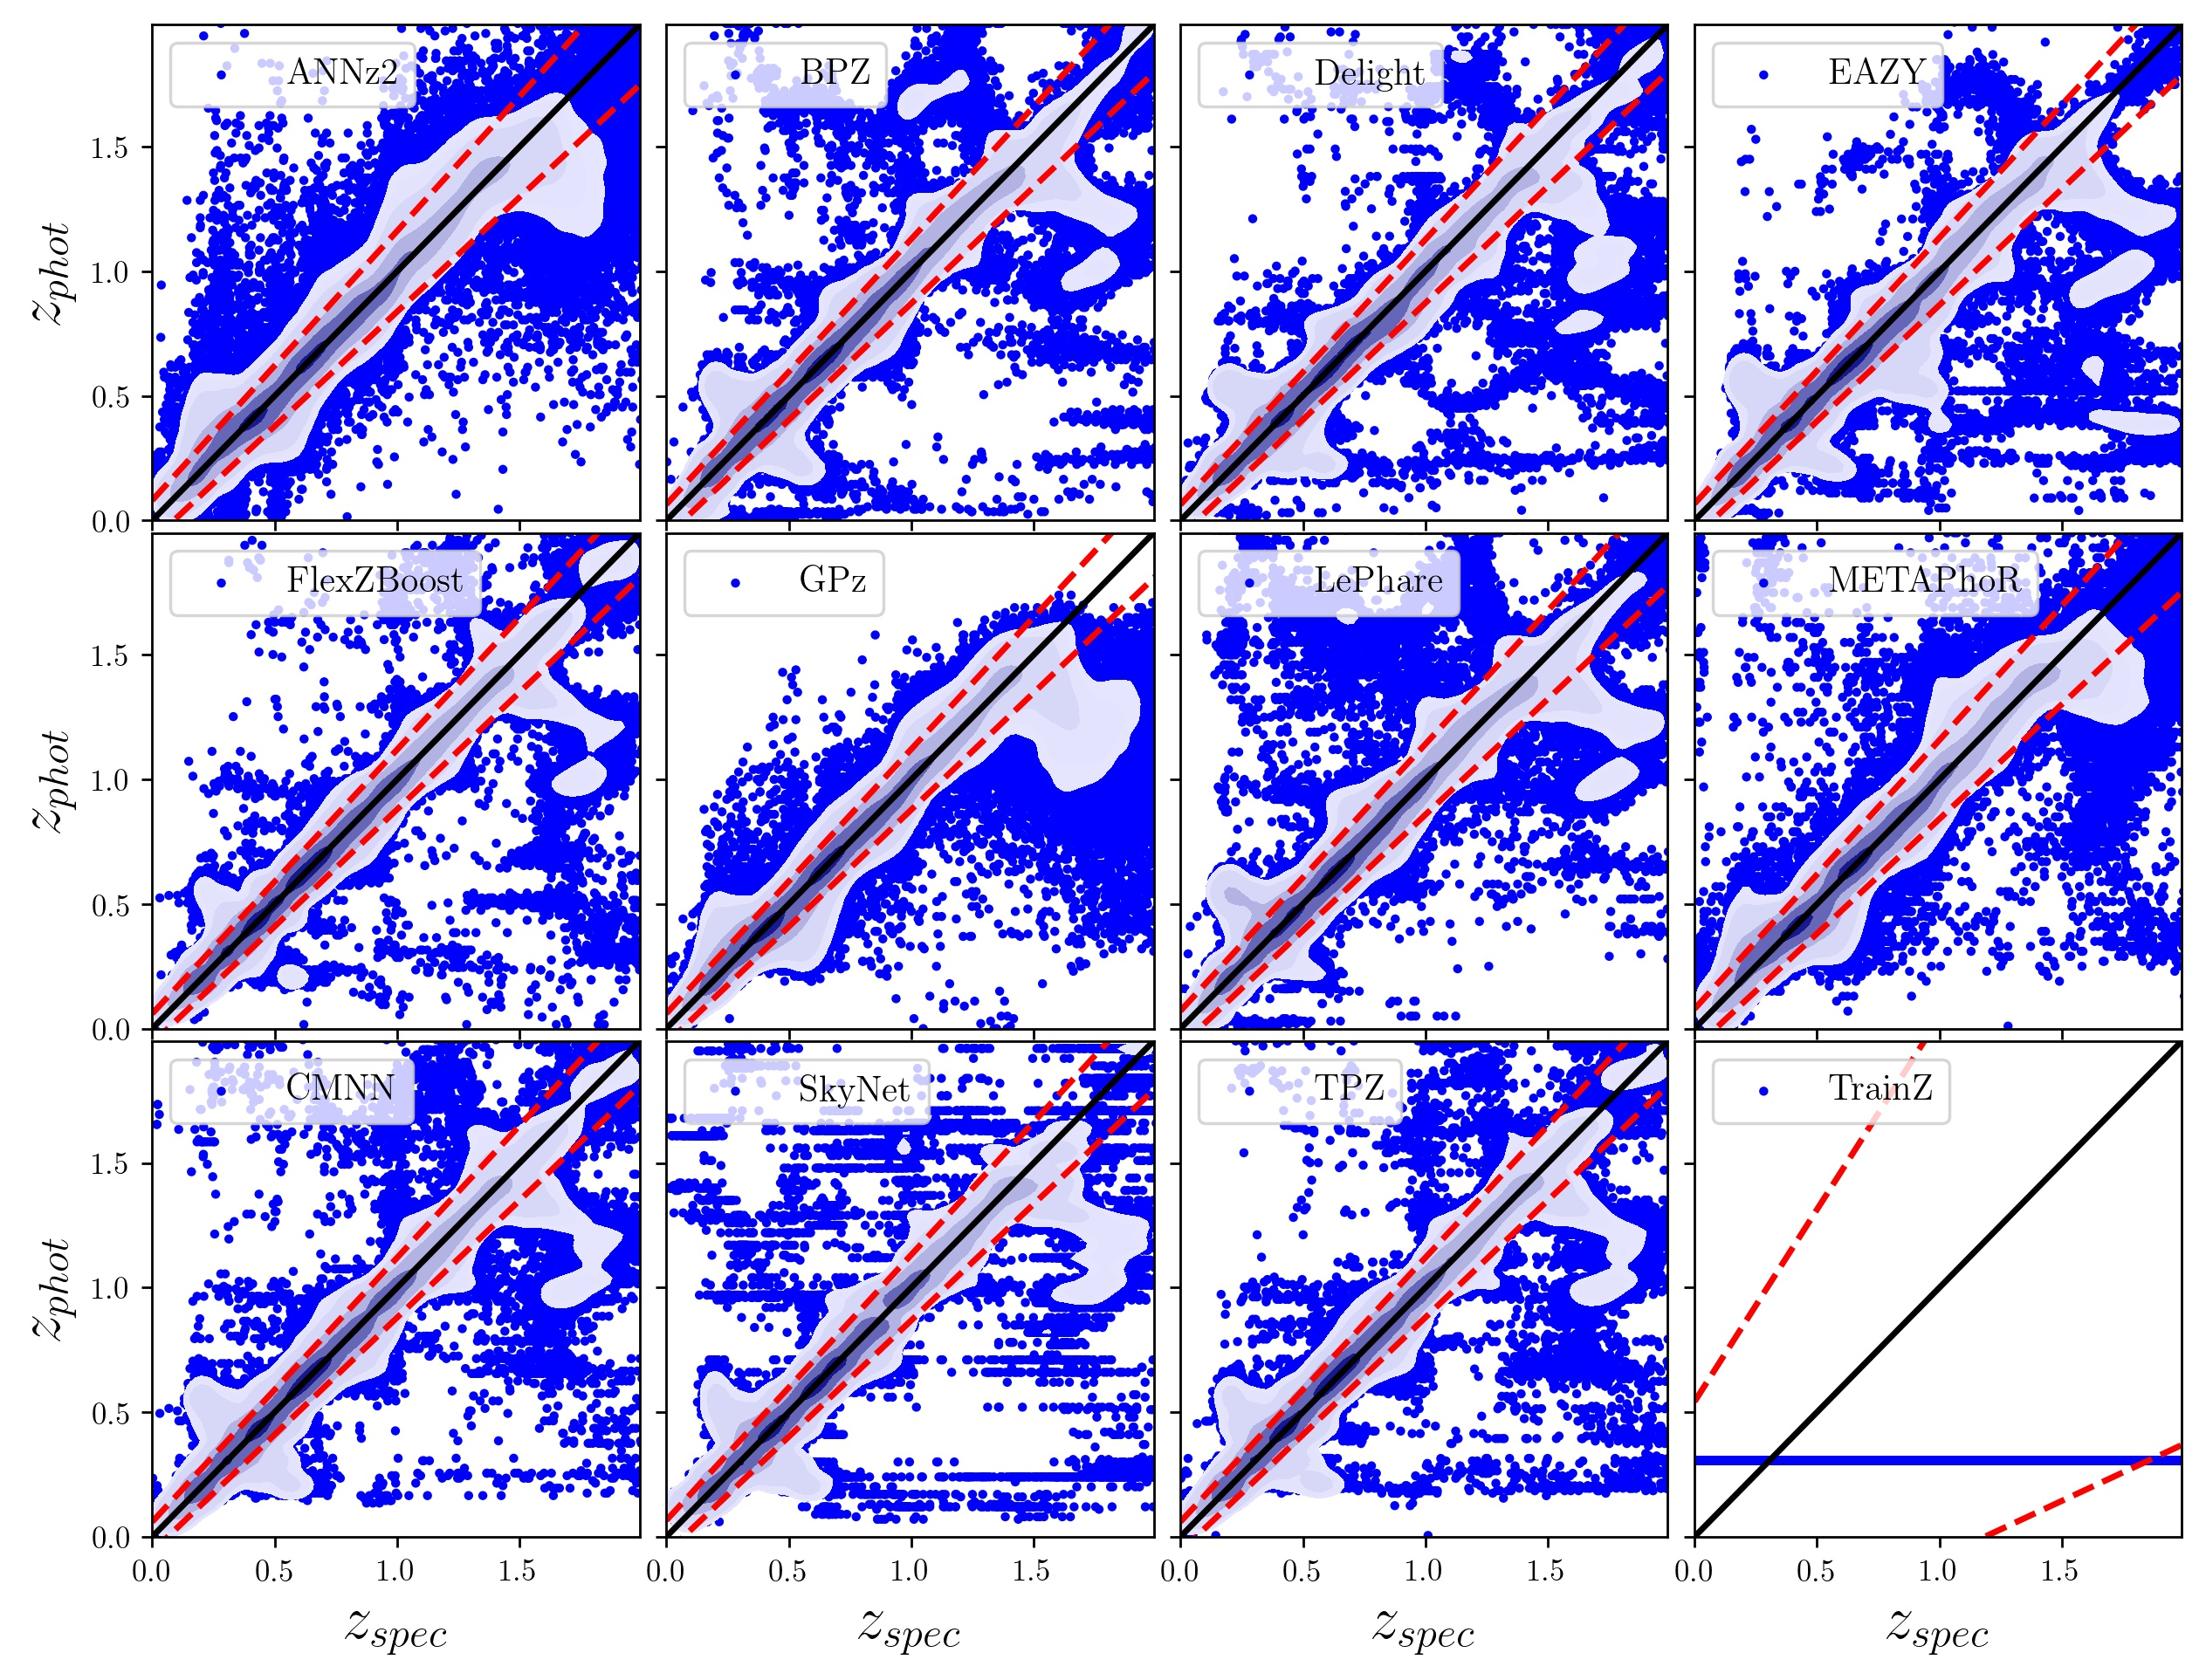
\includegraphics[width=0.9\textwidth]{figures/ZPEAK_szpz_threecolumn_12codes_navy.jpg}
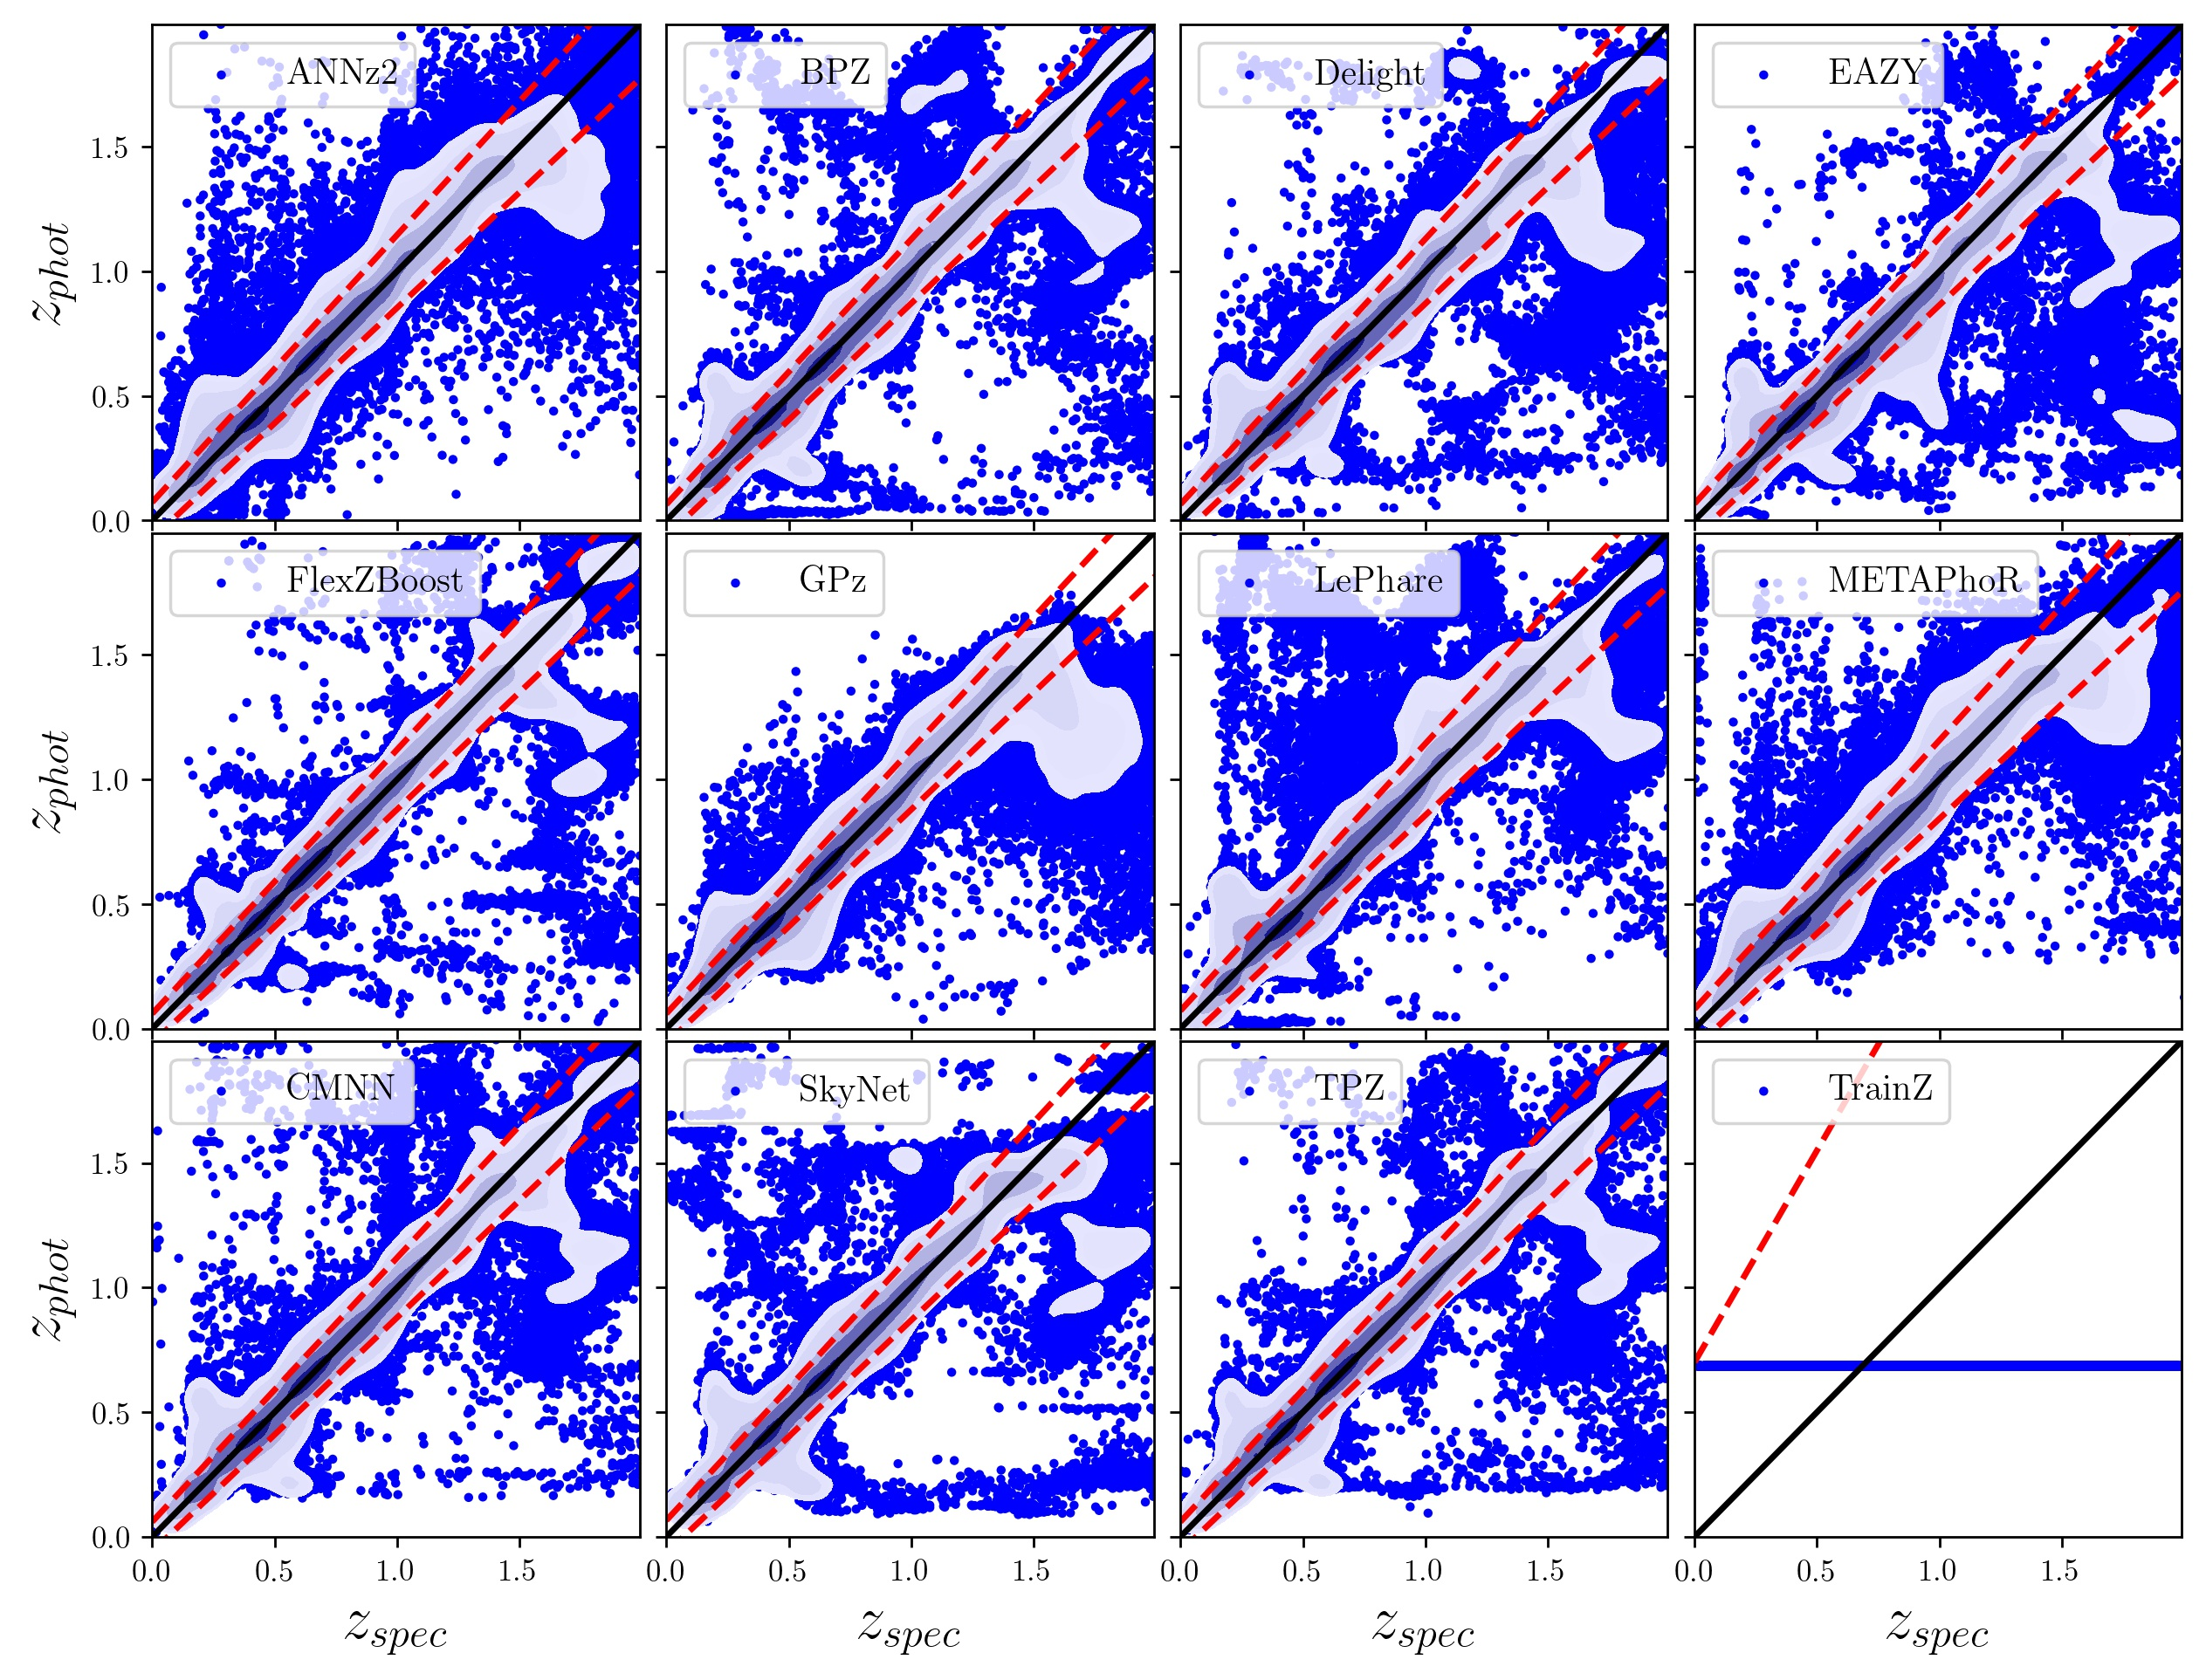
\includegraphics[width=0.9\textwidth]{figures/ZWEIGHT_szpz_threecolumn_12codes_navy.jpg}
\caption{Point estimate photo-z's derived from the posteriors. Top panel shows $z_{PEAK}$, while bottom panel shows $z_{WEIGHT}$.  Point estimate density is represented with fixed density contours, while outliers at lower density are represented by blue points.  While use of point-estimate photo-$z$'s is not recommended, they do make for useful comparative and visual diagnostics.  In the lower-right panel of each plot, the \trainz\ estimator results in identical photo-$z$ estimates at the mode and mean of the training set $N'(z)$ distribution for all galaxies.} \label{fig:pz_pointestimates}
\end{figure*}


\begin{table*}
\begin{center}
\caption{Point estimate statistics}\label{tab:pointestimates}
\begin{tabular}{lcccccc}
\hline
\hline
                  &            & $Z_{PEAK}$  &          &  & $Z_{WEIGHT}$          &\\
\hline
Photo-z Code       & $\frac{\sigma_{IQR}}{(1+z)}$ & median  & \multicolumn{1}{|p{0.75cm}|}{\centering outlier \\fraction} & $\frac{\sigma_{IQR}}{(1+z)}$ & median & \multicolumn{1}{|p{0.75cm}|}{\centering outlier \\fraction}\\
\hline
\textsc{ANNz2}     & 0.0270  &  0.00063  & 0.044      & 0.0244  &  0.000307  & 0.047  \\ 
\textsc{BPZ}       & 0.0215  & -0.00175  & 0.035      & 0.0215  & -0.002005  & 0.032 \\ 
\textsc{Delight}   & 0.0212  & -0.00185  & 0.038      & 0.0216  & -0.002158  & 0.038 \\ 
\textsc{EAZY}      & 0.0225  & -0.00218  & 0.034      & 0.0226  & -0.003765  & 0.029 \\ 
\textsc{FlexZBoost}& 0.0154  & -0.00027  & 0.020      & 0.0148  & -0.000211  & 0.017 \\ 
\textsc{GPz}       & 0.0202  & -0.00091  & 0.036      & 0.0201  & -0.000950  & 0.037 \\ 
\textsc{LePhare}   & 0.0236  & -0.00161  & 0.058      & 0.0239  & -0.002007  & 0.056 \\ 
\textsc{METAPhoR}  & 0.0264  &  0.00000  & 0.037      & 0.0262  &  0.001333  & 0.048 \\ 
\textsc{CMNN}        & 0.0184  & -0.00132  & 0.035      & 0.0170  & -0.001049  & 0.034 \\
\textsc{Skynet}    & 0.0219  & -0.00167  & 0.036      & 0.0218  &  0.000174  & 0.037 \\
\textsc{TPZ}       & 0.0161  &  0.00309  & 0.033      & 0.0166  &  0.003048  & 0.031 \\ 
\hline
\trainz	   & 0.1808  &  -0.2086  & 0.000	  & 0.2335  & 0.022135  & 0.000\\
\end{tabular}
\end{center} 
\end{table*}


\bibliographystyle{mn2e}
\bibliography{references}
\end{document}